\chapter{Introduction\label{chap:intro}}
\renewcommand{\thepage}{\arabic{page}}% Arabic numerals for page
                                      % counter
\setcounter{page}{1}% Start page number with 1



The work presented in this thesis is focused on two important factors
of successfully measuring the neutron Electric Dipole Moment~(nEDM) at
TRIUMF. Those include having a very stable magnetic field environment
as well as high Ultra Cold Neutron~(UCN) statistics. The sensitivity
goal of TRIUMF Advanced Ultracold Neutron source~(TUCAN) collaboration
to measure the nEDM is $10^{-27}$~e$\cdot$cm.


This chapter provides some information on why neutron EDM is
interesting to measure and how finding a nonzero nEDM would answer
questions regarding the matter-antimatter or Baryon asymmetry of the
universe. Chapter~\ref{chap:nedm} gives a brief description of the
future nEDM measurement at TRIUMF and its experimental setup
components. The method of measurement is also presented in that
chapter. Chapter~\ref{chap:muofT} presents the work towards the
dependence of the ambient temperature fluctuations to the internal
magnetic field measured inside the magnetic shielding and find an
upper limit on the temperature stability of the nEDM measurement
environment. Chapter~\ref{chap:UCNattriumf} presents the current UCN
facility at TRIUMF where the where the first UCN was produced with the
vertical UCN source from RCNP and chapter~\ref{chap:UCNresult}
presents the reult of those measurements with UCN. The final remarks
and notes are available in chapter~\ref{chap:overall}.



\section{History of Fundamental Symmetries }

Over the last few decades the interest in the invariance of the
discrete symmetries have been increased. Such studies revealed the
internal structure of the elementary particles and helped develop the
underlying theories.

There are three significant symmetries in physics as Charge
conjugation~($C$), Parity~($P$) and Time-reversal~($T$). $C$-symmetry
simply decribes physical laws under a charge-conjugation
transformation. Parity transformation, is simply the inversion of
spatial coordinates and Time-reversal transformation is changing the
direction of time.  Tests of Charge $C$,$P$ and $T$ symmetries
established the structure
of the Standard Model~(SM)~\cite{pospelov2005electric}.

In 1956, fall of discrete symmetries started with the famous
$\theta-\tau$ paradox in the K-mesons decay. The paradox was that two
particles previously known as $\theta^+$ and $\tau^+$ which had the
same mass and lifetime decayed into products with different parities
\begin{equation}
  \begin{split}
    \theta^+ &\rightarrow \pi^+ + \pi^0 \\
    \tau^+ &\rightarrow \pi^+ + \pi^+ + \pi^-.
  \end{split}
\end{equation}
Initially it was thought that the initial states should also have
different parities but precise measurements revealed that this is not
the case. Yang and Lee suggested that the paradox is originated from
a $P$ violation in the weak
interactions~\cite{lee1957parity}. Immediately after, an experimental
search was suggested by Ramsey for Parity violation in the $\beta$
decay of Co-60. Within a few months, $P$ violation was demonstrated by
three different experiments
~\cite{PhysRev.105.1413,PhysRev.105.1415,friedman1957nuclear}. After
the observation of $P$ violation, Landau showed that Electric Dipole
Moments~(EDMs) are forbidden by $T$
symmetry~\cite{landau1957conservation} and then it was suggested that
$T$ symmetry should also be checked experimentally
\cite{PhysRev.106.517}. 
%In 1964 it was discovered that the $C$ and $P$ symmetries are broken in
%the $K$-meson decay~\cite{christenson1965regeneration}. 

One of the most fundamental symmetries in physics is the
$CPT$~(Charge-Parity-Time) symmetry. The simultaneous operation of
$C$, $P$ and $T$ leaves the system unchanged. To date there is no
experimental evindence for $CPT$ symmetry breaking.  Because of the
$CPT$ invariance, breakdown of $CP$ symmetry should be accompanied by
violation of Time-reversal symmetry. 

A finite EDM provides a good source of $CP$ violation. EDMs caused by
$CP$ violation in the Standard Model are negligible. But most
extensions of Standard Model such as supersymmetry naturally produces EDMs that
are comparable to or larger than present experimental limits.
% ~\cite{romalis2001new}.
The search for EDMs can be traced back to 1950 when Purcell and Ramsey
tested the possibility of finding EDMs for particles and
nuclei. Smith, Purcell and Ramsey started an experiment to search for
neutron EDM $d_n$ and they achieved the upper limit of
$d_n < 5 \times 10^{-20}$~e $\cdot$ cm~\cite{smith1957experimental}.
Over the years the upper limit on the neutron EDM has been improved by
many orders of magnitude. Measurement of particle EDMs provide some of
the tightest constraints on the extensions to the Standard Model to
probe $CP$ violation. The most recent upper limit on the neutron EDM
is found to be $\vert d_n\vert < 3.0 \times 10^{-26} $~e$\cdot$
cm~\cite{pendlebury2015revised}.



\section{Baryon Asymmetry of the Universe}
The neutron EDM provides a highly sensitive diagnostic for $CP$
violation which is an important element for the observed
baryon asymmetry in the universe.  The dominance of matter over
antimatter in the universe can be characterized by~\cite{Cline}
\begin{equation}
\eta = \frac{n_b-\bar{n_b}}{n_{\gamma}} \simeq 6 \times 10^{10}
\end{equation}
where $n_b$ is the number of baryons, $\bar{n_b}$ is the number of
anti-baryons and $n_{\gamma}$ is the number of photons in the Cosmic
Microwave Backgorund.

It is possible to assume that, maybe, the universe is baryon symmetric
in a very large scale and it is split into regions that are made of
only baryons or anti-baryons. If that was the case, an excess of gamma
rays in between these separated regions was expected to be observed
due to annihilation. But, even in the least dense regions of the
space, there is hydrogen gas cloud.

\subsubsection{Sakharov criteria}
There are three key ingredients needed to
create baryon asymmetry known as Sakharov conditions~\cite{Sakharov:1967dj}:
\begin{center}
\begin{description}
\item[$\bullet$]Baryon number violation
\item[$\bullet$] $C$ and $CP$ violation
\item[$\bullet$] Departure from the thermal equilibrium.
\end{description}
\end{center}

The first condition is obvious. It simply means in a reaction, if the
net baryon number is zero, there would be no baryon asymmetry. In the
reactions that violate baryon number, if there is no $C$ and $CP$
violation, the net baryon number would be zero and this is because the
reactions that create excessive baryons will be counter-balanced by
the reactions that create excessive
ani-baryongs.~\cite{theearlyuniverse}.  The third condition is
essential for a net nonzero baryon asymmetry since the equilibrium
average of $B$ vanishes. Sakharov suggested that baryogenesis took
place immediately after the big bang, at a temperature not far below
the Planck scale of $10^{19}$~GeV, when the universe was expanding so
rapidly that many processes were out of thermal
equilibrium~\cite{cohen1993progress}.




\section{Neutron Electric Dipole Moment and Symmetry Breaking}
A permanent neutron EDM is an intrinsic property of a neutron. This
fundamental property is a measure for the separation of positive and
negative charges internal to the neutron. However, no nEDM has been
measured so far.

The interaction of a nonrelativistic neutron with
the electromagnetic field can be descibed by the follwoing
hamiltonian:

\begin{equation}
  \label{eqn:hamiltonian}
 H= -\boldsymbol{\mu_n} \cdot \bf{B} - \bf{d}_n \cdot \bf{E}
 \end{equation}
where $\boldsymbol{\mu}_n$ is the magnetic moment of the neutron
interacting with the magnetc field $\bf{B}$, and $\bf{d}_n$ is
the electric dipole moment of the neutron interacting with the
electric field $\bf{E}$.

The properties of the Hamiltonian under discrete symmetries is
summarized in Tab.~\ref{tab:Hsymmetry}. Based on this, the first term
is $CP$-even and $T$-even and the second term is $cp$-odd and
$T$-odd. Because of the $CPT$-invariance, a nonzero EDM may exists if
both Parity and Time-reversal symmetries are broken.


\begin{table}[h!]
  \label{tab:Hsymmetry}
\begin{center}
\begin{tabular}{| l | l | l | l |} 
\hline
 & C & P & T \\ \hline
\textbf{B} & - &+ &- \\ \hline
\textbf{E} & -&- &+ \\ \hline
$\boldsymbol{\mu}$ &- &+ &- \\ \hline 
\textbf{d} & -&+ &- \\ \hline
\end{tabular}
\caption{Symmetry properties of different components of the EDM Hamiltonian}
\end{center}
\end{table}
  
The nEDM measurement technique and a breif survey of the current nEDM
measurement sites worldwide are presented in chapter~\ref{chap:nedm}.



%\subsection{Physics Beyond the Standard Model}



\section{Ultracold Neutrons}
The measurement of the nEDM is strongly correlated with having high
neutron statistics. Table~\ref{tab:ucnenergy} shows the energy regime
of neutrons and their corresponding velocity, temperature and de
Broglie wavelength via
\begin{equation}
  \label{eqn:ucnenergy}
  E = \frac{1}{2} m v^2 = \frac{3}{2} k_B T = \frac{h^2}{2m \lambda^2}
\end{equation}
where $m$ is the mass of the neutron, $v$ is the neutron velocity,
$k_B$ is Boltzmann constant, $T$ is the equivalent temperature, $h$ is
Planck's constant and $\lambda$ is de Broglie wavelength.

\begin{table}
  \label{tab:ucnenergy}
  \centering
  \begin{tabular}{|c|c|c|c|c|}
    \hline
    Name & Energy $E$ & Velocity $v$ & Temperature $T$ & Wavelength $\lambda$ \\
    \hline
    \hline
    Fast & 10~MeV & $4.4 \times 10^7$~m/s & $7.7 \times 10^{10}$~MK & 9.0~pm \\
    \hline
    Thermal & 0.0254~eV & $ 2.2 \times 10^3$~m/s & 290~K & 0.2~nm \\
    \hline
    Cold & 1~meV & 500~m/s & 8~K & 3~nm \\
    \hline
    Ultracold & 300~neV & 8~m/s & 3~mK & 50~nm \\
    \hline
  \end{tabular}
  \caption{Commonly used names for neutrons in different energy ranges
    and their corresponding velocity, temperature and wavelenght}
\end{table}



Ultracold Neutrons~(UCN) are neutrons with kinetic energy
$\lesssim 300$~neV corresponding to a velocity of~$\lesssim 8$~m/s or
temperatures $\lesssim 3$~mK. UCN move so slowly that they can
populate traps made of matter, magnetic and gravitational fields and
can be stored and manipulated for several hundreds of seconds in such
traps. Because of this property, UCN are a valuable tool for precise
measurements in fundamental physics.

% such as studies of quantum states of the neutron in the Earth's
% gravitational field or the measurement of the neutron EDM.
High precision studies of the static and decay properties of the
neutron and its interactions provide important data for particle
physics and cosmology. In addition, they enable sensitive searches for
new physics. Examples of the experiments using UCN which aim to
discover new physics are searches for a permanent electric dipole
moment (EDM) of the
neutron~\cite{Baker2006,Serebrov2009,Lam_Gol,Altarev2010,Pendlebury2015},
precision measurements of the neutron
lifetime~\cite{Paul2009,Wietfeldt2011,Arzumanov2000,Serebrov2005,Huffman},
and $\beta$-decay correlation parameters~\cite{Mendenhall,Broussard},
as well as quests for dark matter
candidates~\cite{Ben2007,Serebrov2008,Zimmer2010}, axion-like
particles~\cite{Baessler,Serebrov2010,Jenke2014,Afach2015}, Lorentz
invariance violations~\cite{Altarev2009} and the measurements of the
quantum states of UCN in the gravitational field of the
earth~\cite{Nesvizhevsky2003}.

%Among recent new topics addressed with UCN feature searches for
%‘‘mirror matter’’ as a viable candidate for dark matter, a sensitive
%test of Lorentz invariance, searches for a new fundamental force
%mediated by axionlike particles, and a demonstration of the effect of
%accelerated matter on the neutron wave.  More long-standing are
%efforts to improve the accuracy of the weak axial-vector and vector
%coupling constants of the nucleon derived from precise values of the
%neutron lifetime and the beta asymmetry, i.e., the asymmetry of
%electron emission with respect to the spin of the decaying
%neutron. These values crucially enter the calculation of reaction
%rates in big-bang nucleosynthesis and stellar fusion [16]. They are
%also applied to calculate various processes in particle physics such
%as for the calibration of antineutrino detectors, which is currently
%scrutinized in view of a ‘‘reactor antineutrino anomaly’’ hinting at
%the existence of sterile neutrinos [17,18].

The neutron is an electrically neutral hadron and participates in all
of the four fundamental interactions as described below.



%~\cite{beatrice,knecht,golub1994neutron,golub1991ultra}:


\subsubsection{The Gravitational Interaction}
The neutron has a mass $m_n\approx 940$~MeV/c$^2$ and therefore has a
potential in the Earth's gravitational field
\begin{equation}
V_g=mgh
\end{equation}
where $h$ is the vertical displacement and $g=9.8$~m/s$^2$ is the
acceleration due to the earth's gravitational field.  In experiments
using thermal or cold neutrons, the effects of gravity can usually be
negligible due to the short survival times of the neutrons. However,
with UCN experiments, since they are confined for up to several
hundred seconds, gravity has a significant influence.

Here
\begin{equation}
mg=102\; \text{neV/m}
\end{equation}
which is comparable to the UCN kinetic energy. This means a UCN of
energy 200~neV can rise by at most 2~m.

\subsubsection{The Weak Interaction}
The weak interaction governs the radioactive $\beta$-decay of
neutrons. UCN decay into a proton, an electron and an electron
antineutrino via
\label{neutrondecay}
\begin{equation}
n\longrightarrow p+e^{-}+\bar{\nu_{e}}.
\end{equation}
The value of neutron lifetime sets the maximum time constant with
which UCNs can be stored for. The current value of the neutron
lifetime is $880.3 \pm 1.1$~s~\cite{PDG2016}.

\subsubsection{The Electromagnetic Interaction}

Neutron is an electrically neutral, spin-1/2 particle that possesses a
magnetic dipole moment due to its internal structure through which it
interacts with a magnetic field \textbf{B} as
\begin{equation}
  \label{eqn:vmag}
V_m=-\boldsymbol{\mu}_n \cdot \textbf{B}
\end{equation}
where
\begin{equation}
\vert \boldsymbol{\mu}_n \vert =60 \; \text{neV/T}.
\end{equation}

In an inhomogeneous magnetic field, UCN experience a force described
by the following equation
\begin{equation}
  \label{eqn:fmag}
  \bf{F_m} = - \boldsymbol{\nabla}V_m = \pm \vert \boldsymbol{\mu_n} \vert \boldsymbol{\nabla} \bf{B}.
\end{equation}
In the nEDM measurement, the interaction of UCN with the magnetic
field is used to polarize UCN and to measure its polarization at the
end of the measurement cycle~(see Sec.~\ref{sec:Ramsey}).  In
Eqn.~\ref{eqn:fmag} the sign $\pm$ corresponds to the relative
orientation between the magnetic moment and the magnetic field.  UCN
of anti-parallel spin to the magnetic field~(magnetic moment parallel)
called {\it{high field seekers}} have negative $V_m$, accelerate
towards strong magnetic fields and are attracted to it and UCN with
parallel spin~(and thus magnetic moment anti-parallel) to the magnetic
field called {\it{low field seekers}} have positive $V_m$ and are
repelled by it.  Eqn.~\ref{eqn:fmag} is true only if UCN moves
adiabatically through the magnetic fields. This condition will be
fulfilled when the Larmor precession frequency of UCN is smaller than
the changes in the magnetic field in the rest fram of UCN. However,
since UCN have low speeds, this condition is easily fulfilled.  If the
UCN spin adiabatically traces the magnetic field, it will be fully
polarized which can be achieved by passing UCN through a
strong~$\sim 6$~T magnetic field.

%If the magnetic field $\textbf{\textit{B}}$ is inhomogeneous and the
%neutron spin traces the magnetic field adiabatically, the neutron will
%experience a force given by:

%\begin{equation}
%\label{eqn:emforce}
%\textbf{\textit{F}}_{mag}= - \mathbf{\mathit{\nabla}} V_{mag}=\pm
%\mu_n \mathbf{\mathit{\nabla}} \vert \textbf{\textit{B(r)}} \vert.
%\end{equation}
%The neutrons that experience a force towards regions of higher
%magnetic field strength are called high-field seekers. Conversely if
%the neutrons experience a force towards regions of lower magnetic
%field (a 3D minimum in the $\textbf{\textit{B}}$ field) strength they
%are called low-field seekers. It is this force that allows UCN with
%sufficiently low energy to be confined by magnetic field gradients.
%%If the UCN spin adiabatically traces the magnetic field, it will be fully polarized
%%which can be achieved by passing UCN through a strong $\sim$~6~T magnetic field.
%Furthermore, Nuclear Magnetic Resonance (NMR) experiments can be
%conducted on UCN. For example, NMR is used to measure the EDM of
%neutrons (the Ramsey technique) where UCN are placed in aligned
%electric and magnetic fields.


\subsubsection{The strong Interaction}
The neutrons and protons are bound in the nucleus by the strong
interaction. However, this interaction has a short range and it only
affects the neighbouring nuclei.
The Woods-Saxon potential approximately
describes the nucleons interaction inside the atomic nucleous
\begin{equation}
  \label{eqn:woodsax}
  V(r) = - \frac{V_0}{1+\exp(\frac{r-R}{a})}
\end{equation}
where $V_0$ represents the potential well depth, $a$ represents the
surface thickness of the nucleous and $R = r_0 A^{1/3}$ where
$r_0 = 1.25$~fm and $A$ is the mass number. For neutrons and protons
the depth is $V \approx -40$~MeV. The UCN energy and its binding
energy and the depth of the potential differ by many orders of
magnitude. As a result, it is not possible to use perturbation theory
to describe neutron scattering. Fermi realized that it is possible to
introduce an equivalent potential which can be used to calculate the
small changes in the wavefunction outside the range of the interaction
by perturbation theory.

The interaction of an incident neutron with a liquid or a solid could
be described by sum of $\delta$ functions

\begin{equation}
  \label{eqn:vFermi}
  V(r) = \frac{2\pi \hbar^2}{m_N} \sum_i a_i \delta (r - r_i)
\end{equation}
where $m_N$ is the mass of neutron, $r_i$ is the position of ith
nucleus and $a_i$ is the scattering length with the ith
nucleus. Because of UCN's large wavelength this equation can be
written as
\begin{equation}
V(r) = \frac{2\pi \hbar^2}{m_N}\sum_i N_ia_i
\end{equation}
where $N_i$ is the number density in the material i. In UCN physics
this potential is typically called neutron optical potential since if
the energy of the neutron is less than the optical potential $E < V$
the neutron will be fully reflected from the material surface under
any angle of incidence. This sets a limit on the UCN velocity.

UCN can be lost when it is reflected from the material walls and the
it is because of the upscattering in which UCN absorbs energy or
absorption in which UCN gets absorbed by the nucleus of the reflecting
material. To include the losses in the potential, the optical
potential is usually written as
\begin{equation}
  U(r) = V(r) - iW.
\end{equation}
The ratio $\eta = V/W$ is a measure of the loss per bounce probability
of the material. 

The strong interaction plays a crucial role in the nEDM
measurement. Choosing certian materials enables us to store and guide
UCN to the measurement cell.  The highest known value for the optical
potential is $V_F=335$~neV and is measured for $^{58}$Ni.

%\subsection{Superthermal Sources of Ultracold Neutrons}



%The search for a nonzero neutron EDM provides a promising route to
%investigate new mechanisms of CP violation beyond the standard
%model. These in theory could help explain the matter-antimatter
%asymmetry in the Universe. At the present best level of sensitivity
%$d_n = 3.0 \times 10^{-26}$~e$\cdot$cm (90\%
%C.L)~\cite{Pendlebury2015} which was limited by counting
%statistics, severe constraints on new sources of CP violation were
%placed.

%As most other experiments with UCNs, the EDM search has been
%performed using a long-serving source~\cite{Steyerl1986} at the
%high-flux reactor of the Institut Laue Langevin (ILL) in Grenoble,
%France. It employs a neutron turbine for a phase-space transformation
%of very cold neutrons from a liquid deuterium moderator down to the
%energy range of UCN, whose high-energy limit is set by the neutron
%optical potential of the material selected for a UCN trap (such as
%252 neV for beryllium) or by the magnetic potential provided by field
%gradients in a magnetic bottle (60 neV=T). With UCN densities in the
%order of 10 per cm3 made available for experiments in a typical
%configuration of the UCN extraction from the turbine [23], the ILL
%source has defined the state of the art for more than 25
%years. However, notably,
%%%%%%%%%%%%%%%%%%%%%%%%%%%%%%%%%%%%%%%%%%%%%%%%%%%%%5
%The prospect to make an important discovery in refining the neutron
%EDM search has strongly motivated many research groups to develop next
%generation UCN sources~\cite{Golub75,Zimmer2011} which aim to
%improve the available UCN densities by more than 2 orders of
%magnitude.
%%%%%%%%%%%%%%%%%%%%%%%%%%%%%%%%%%%%%%%%%%%%%%%%%%%%%%%%%%%5
%\subsection{Properties of UCN}
%expand the first two paragraphs of Leung's paper. Also look at
%Leung's thesis.  Neutron energy and its velocity are related as
%$E_n=\frac{m_n v^2}{2}= \frac{\hbar^2 k^2}{2 m_n}=\frac{h^2}{2 m_n
%\lambda_n^2}$ where $m_n$ is the neutron mass, $v$ is the neutron
%velocity and $k=\frac{2 \pi}{\lambda_n}$ is the wave number. The
%kinetic energy is related to temperate as $E_n=k_B T_n$ where $k_B$
%is the Boltzmann constant.

%UCN have velocities less than 8~m/s and energies about 260~neV which
%corresponds to temperatures below 2~mK.  The kinetic energy of UCN is
%less than the neutron optical potential of well-chosen materials and
%so they can reflect from material surfaces at all incident angles,
%allowing them to be stored in a vessel and studied for times
%approaching the neutron lifetime.



\section{Superthermal UCN sources}
\label{sec:ucn_with_heII}



In thermal UCN sources neutrons are extracted from a
distribution almost in thermal equilibrium with a moderation system.
The UCN turbine source at the Institute Laue-Langevin~(ILL) extracted
very cold neutrons vertically from a cold source~(liquid deuterium)
and slowed them down using the mechanical action of a
turbine~\cite{Steyerl1986,Steyerl1975}. Here cold neutrons
with velocities of $\sim$~40~m/s are decelerated by reflection from a
set of curved turbine blades moving with a velocity $\sim$~20~m/s in
the same direction as the neutrons. A UCN density $\sim$~40~UCN/cm$^3$
was achieved with this method~\cite{ucnbook,Albert_talk}. %The
current UCN density of this source is 110~UCN/cm$^3$ for neutrons with
velocities $<$~7m/s\cite{Steyerl1986}.


%\subsection{Goals of Superthermal UCN Sources}
In 1975 it was shown that, it is possible to achieve higher steady
state UCN densities corresponding to temperatures much lower than the
temperature of the moderator~\cite{Golub75}. These are called
superthermal converters. Here thermal or cold neutrons are
inelastically scattered and transfer their kinetic energy to an
excitation of the converter medium ({\it{e.g.}} to a phonon).
Superthermal sources have the ability to provide much higher UCN
densitys (i.e. more UCN) than conventional sources such as the ILL
turbine source.  The best candidates for superthermal converters to
date are solid deuterium and liquid $^4$He.


%UCN are a powerful tool to study new physics and the properties of
%the neutrons.  An intense UCN beam is a common need for all of these
%experiments.  Producing a high intensity UCN source is an essential
%need for such studies.  Earlier method Before using superthermal
%converters, UCN were produced by neutron turbine
%sources~\cite{Steyerl1986,Steyerl1975}. In turbine source,
%cold neutrons with velocities of $\sim$ 40~m/s are brought into UCN
%range by reflection from a set of curved turbine blades moving with a
%velocity $\sim$ 20~m/s in the same direction as the neutrons. A UCN
%density of $\sim$30-40 UCN/cm$^3$ was achieved with this
%method~\cite{ucnbook}.

%In earlier methods of UCN production, it was assumed that the maximum
%UCN density would be achieved if the incident neutron flux is
%thermalized to the moderator~\cite{Shapiro}. The maximum
%achievable UCN density with these methods is
%$10^2-10^3$/cm$^3$~\cite{ucnbook}. The process of extracting UCN
%has a considerable degree of loss, which means, the available UCN
%will always be much less than this~\cite{ucnbook}.  The low
%density of UCN produced by thermal sources was the main constrain of
%high precision measurements such as neutron $\beta$-decay with
%UCN~\cite{Huffman} and neutron electric dipole moment
%measurement~\cite{Steyerl1986,Harris99}.

 
\subsection{Basic Idea of Superthermal UCN Sources\label{sec:basic_idea}}
The mechanism of a superthermal UCN source is the following.  An
incident neutron can lose almost its entire energy in a single
scattering event by creating excitations ({\it e.g.} phonons) in a
converter medium~\cite{ucnbook, Golub75}. Because of the loss
in the kinetic energy, this process is called downscattering. The
reverse process is called upscattering where a UCN absorbs kinetic
energy from the medium.


Consider a simple model for the medium as a two-level system with an
energy gap $E_0^*$.  A neutron can excite a quasi-particle from the
lower state to the higher state by transferring the energy $E_0^*$. A
quasi-particle from the higher state can fall down to the lower state
by transfer of the energy $E_0^*$ to a neutron.  The principle of
detailed balance links the cross-section for upscattering
$\sigma(E_{\text{UCN}} \rightarrow E_{\text{UCN}}+E_0^*)$ and downscattering
$\sigma(E_{\text{UCN}}+E_0^* \rightarrow E_{\text{UCN}})$~\cite{ucnbook}

\begin{equation}
\label{eqn:detailed_balance}
\sigma(E_{\text{UCN}} \rightarrow E_{\text{UCN}}+E_0^*)= \frac{(E_{\text{UCN}}+E_0^*)}{E_{\text{UCN}}}
e^{-\frac{E_0^*}{k_B T}}\sigma(E_{\text{UCN}}+E_0^* \rightarrow E_{\text{UCN}})
\end{equation}
where $T$ is the temperature of the medium, $E_{\text{UCN}}$ is the
energy of the UCN, and $k_B$ is the Boltzmann constant.

In general $\sigma(E_{\text{UCN}}+E_0^* \rightarrow E_{\text{UCN}})$ is practically
independent of $T$ so that for $E_0^* \gg k_B T \gg E_{\text{UCN}}$ the
upscattering cross-section for UCN can be made arbitrarily small by
decreasing the temperature. If the converter is now placed in a
neutron flux at a temperature $T_n \geq E_0^*$ there will be a
significant number of downscattering events and a negligible number of
upscattering events.

If the converter is contained in a vessel whose walls are good UCN
reflectors with potential $V \gg V_m$ where $V_m$ is the UCN potential
of the converter, and the walls are transparent to the neutrons of
energy $E_0^*$, then UCN will build up in the moderator to a density
until the rate of loss is equal to the rate of UCN production.

%Coherent inelastic scattering can provide the equivalent of a
%two-level system for UCN \cite{ucnbook}.  A neutron at rest can
%only absorb a phonon with energy E$_0^*$ and a neutron with
%E$>$E$_0^*$ can come to rest by emitting a phonon with energy
%E$_0^*$.  The upscattering process is suppressed by a Boltzmann
%factor $e^{-E_0^*/{k_BT}}$. If the medium is sufficiently cold and
%the excitation energy introduced by the neutrons can be cooled away,
%upscattering becomes negligible.  If the converter is at thermal
%equilibrium at temperature $T$, then $E_0^* \gg k_B T \gg E_{\text{UCN}}$
%where $E_{\text{UCN}}$ is the UCN energy. Only neutrons with energies close
%to $E_0^*$ can scatter in the converter medium. In addition, the UCN
%bottle wall has to have a much higher effective potential than the
%converter medium to prevent UCN loss.

The steady state UCN density in the source is given by
\begin{equation}
\label{ucndensity}
\rho_{\text{UCN}}=P_{\text{UCN}} \tau
\end{equation}
where $P_{\text{UCN}}$~(UCN/cm$^3 \cdot$s) is the UCN production rate
and $\tau$~(s) is the UCN mean lifetime in the system.  The mean
lifetime $\tau$ of the UCN in the vessel is restricted by a variety of
possible loss mechanisms
\begin{equation}
\frac{1}{\tau} = \frac{1}{\tau_a}+ \frac{1}{\tau_W}+\frac{1}{\tau_{up}}+\frac{1}{\tau_{\beta}}
\end{equation}
where $1/\tau_a$ is the UCN absorption rate in the medium, $1/\tau_W$
is the rate of the UCN loss on the walls, $1/\tau_{up}$ is the neutron
loss due to the upscattering in the medium and $1/\tau_{\beta}$ is the
$\beta$-decay losses.

%An important factor in choosing a UCN source is the absorption rate of the neutron. As a result, pure
Pure deuterium and liquid $^4$He are good candidates for superthermal
conductors, possessing a balance of high production rate and small
neutron absorption cross-section and upscattering rate.


\subsection{UCN Production by Superfluid $^4$He}

\subsubsection{Superfluid $^4$He Definition}

$^4$He is an isotop of helium with two protons and two neutrons. It
has an integer spin of zero which makes it a boson. As a result, it
follows the Bose-Einstein statistics. It has two liquid states known
as He-I and H-II. The He-I phase is the normal fluid phase and He-II
is the superfluid phase with zero viscosity and zero
entropy. Fig.~\ref{fig:phasetransition} shows the phase transition
diagram of $^4$He. These two phases are separated out by the
$\lambda$-line. The phase transition happens at 2.172~K.  Below the
lambda line the liquid can be described by the so-called two-fluid
model which consists of both phases. Below 1~K the liquid is mostly
superfluid.

\begin{figure}[h!]
  \centering 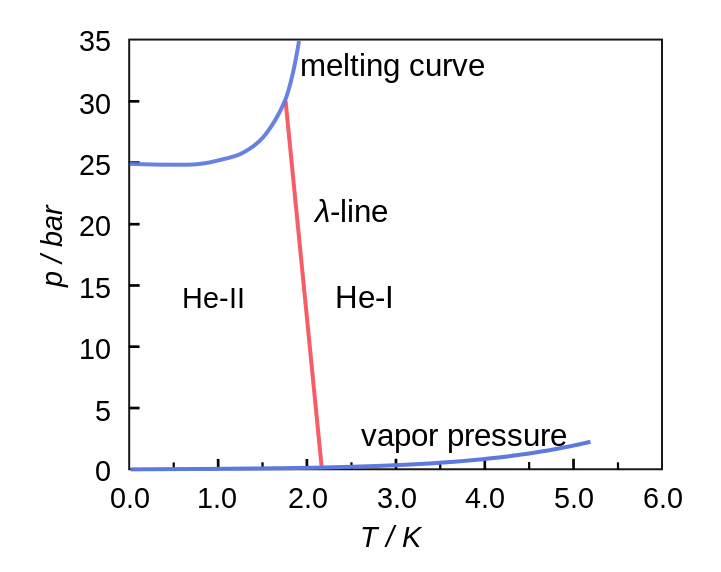
\includegraphics[width=0.7\textwidth]{phasetransition.png}
  \caption{The phase diagram of $^4$He. Here the normal fluid phase or
    He-I and the superfluid phase or H-II are shown.}
\label{fig:phasetransition}
\end{figure}

Because of its zero viscosity, superfluid helium has the ability to
flow through very small capillaries or narrow channels without
experience any friction at all. The flow of liquid helium along the
surface is called {\it{film flow}}.

 
%%%%%%%%%%%%%%%%%%%%%%%%%%%%%%%%%%%%%%%%%%%%%
\subsubsection{Superfluid Helium Converter}

The superfluid $^4$He is an attractive candidate as a UCN source and
was studied in Ref.~\cite{Golub77}.  It has zero neutron absorption
cross-section resulting in $\tau_a \rightarrow \infty$ which makes it
a good candidate as a UCN source.  In superfluid helium, upscattering
losses become smaller than $\beta$-decay losses below $T \sim 0.7$~K.
The dominant production mechanism is the excitation of a single phonon
at the crossing of the free neutron and phonon dispersion curves, with
a momentum $q\sim 0.7$/\AA~\cite{Brome2001} and energy 1~meV
corresponding to a neutron wavelength 8.9~\AA. The availability of
8.9~\AA~cold neutrons is crucial and their flux must be maximized.
%For a long UCN lifetime in superfluid helium, besides the low
%temperature of the converter, the $^3$He contamination must be low
%($^3$He/$^4$He $\le 10^{-12}$), due to its large absorption
%cross-section, which requires $^4$He purification.
There are two types of UCN sources based on superfluid helium: sources
where experiment and source are combined in one apparatus and the
measurement is performed inside the superfluid helium, and
extracted-UCN sources where the source is an apparatus on its own and
delivers neutrons to experiments at room temperature connected to it
by UCN guides.



\subsubsection{UCN Production Rate with Single Phonon scattering in
  Superfluid
  helium~\cite{Korobkina2002,Schmidt2009,Golub77}\label{sec:UCN_production}}
UCN can be produced by one phonon excitation in superfluid helium when
the energy of the incident neutrons is equal to that of the one phonon
excitation in the medium. The incident neutrons then scatter down to
UCN by creating one-phonon excitations in the converter medium.
%The crossing of the dispersion curve for excitations in superfluid
%helium and the free energy of the neutron shows that the neutron
%wavelength should be 0.89~nm~\cite{Brome2001} or 8.9~\AA ~in
%order to excite phonon transitions.
\begin{figure}[h!]
\begin{center}
   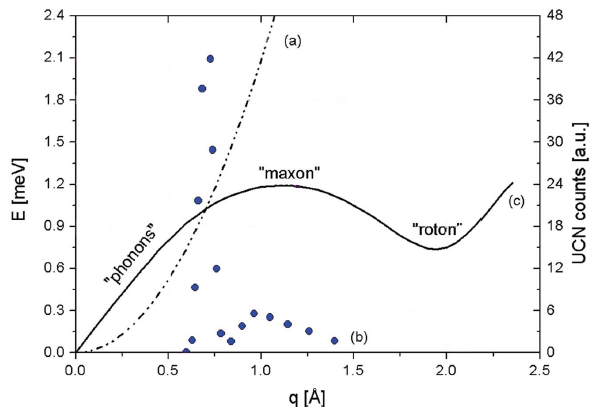
\includegraphics[width=0.7\textwidth]{FIG1_2.PNG}
    \caption{\cite{PSI_news} Dispersion relation of superfluid
      helium (c) and of the free neutron (a). Neutrons with $E\simeq
      1$~meV and wavenumber $q \simeq 0.7$/\AA~can excite a single
      phonon with the same energy and momentum and be downscattered to
      UCN energy range. The UCN production rate (b)(circles) shows the
      dominance of this single phonon process with respect to
      multiphonon processes at higher momentum $q$.
%    The two curves cross at $q=0$ and at $q=q^*$, which corresponds
%    to a neutron wavelength of 0.89~nm, oe an energy of 12~K.
    }
%     \vspace{-2.em}
    \label{fig:FIG1}
    \end{center}
\end{figure} 
Fig.~\ref{fig:FIG1} shows the dispersion relation of the superfluid
helium and a free neutron. A neutron at rest can absorb energy $\hbar
\omega$ and momentum $\hbar q$ with
\begin{equation}
\label{neutron_energy}
\omega=\frac{\hbar q^2}{2m}
\end{equation}
where $m$ is its mass of the neutron. A neutron with this energy and momentum can
come to rest after transferring its energy and momentum to the
superfluid $^4$He. For single phonon interactions, which are usually
dominant, the superfluid can only exchange quantities of energy and
momentum that are related by the dispersion curve

\begin{equation}
\label{dispersion_helium}
\omega=\omega(q)= cq
\end{equation}
where $\omega$ is the energy of the phonon, $q$ is the phonon's
momentum, and $c$ is the speed of sound in the moderator. The second
equal sign in Eqn.~(\ref{dispersion_helium}) is an approximation to
simplify the discussion. The neutrons can only come to rest by
emission of a single phonon if they have the resonant energy $E_0^*$
given by the intersection of Eqns.~(\ref{neutron_energy}) and
(\ref{dispersion_helium})

\begin{equation}
\omega(q)=cq=\frac{\hbar q^2}{2m}
\end{equation}
and so
\begin{equation}
q^*=\frac{2mc}{\hbar}.
\end{equation}

%Fig.~\ref{fig:FIG1} shows that an incident neutron can lose its
%entire energy by creating a phonon excitation inside the converter
%medium if it has the energy amount equal to the phonon excitations in
%the converter medium. If this energy is $E_0^*=\hbar^2 k_0^*/2m$,
%using Eqns.~(\ref{dispersion_helium}) and~(\ref{neutron_energy}),
%$k_0^*=2mc/ \hbar$.

The differential cross-section for neutron scattering is given by the
dynamic scattering function $S(q,\omega)$ which is the Fourier
transform of the Van Hove correlation function $G(r,t)$ in space and
time of the superfluid helium~\cite{Squires}:

\begin{equation}
\frac{d\sigma}{d\omega}=b^2 \frac{k_2}{k_1}S(q,\omega) d\Omega
\end{equation}
where $b$ is the bound neutron scattering length for $^4$He,
$\hbar k_1$ is the momentum of the incident neutrons and
$\hbar k_2=\hbar k_{\text{UCN}}$ is the momentum of UCN. The quantity
$S(q,\omega)$ has been measured in great
detail~\cite{S_func1,gibbs1999collective,S_func3}. Performing the
change of variables,

\begin{equation}
d\Omega=2 \pi \sin \theta d \theta = 2 \pi \frac{q dq}{k_1 k_2}
\end{equation}
gives

\begin{equation}
 \frac{d\sigma}{d\omega}=2\pi b^2 \frac{k_2}{k_1}S(q,\omega)\frac{q
   dq}{k_1 k_2}=2\pi b^2 S(q,\omega)\frac{q dq}{k_1^2}.
\end{equation}
This may effectively be integrated over the limits on $q$ which are

\begin{equation}
k_1-k_2 < q < k_1+k_2.
\end{equation}
Since
\begin{equation}
k_2=k_{\text{UCN}} \ll k_1, \; \; \; \; q\sim k_1 
\end{equation}
we may write $dq=2k_{\text{UCN}}$. This results in the cross-section
being related to $S(q,\omega)$ evaluated on the incident neutron's
dispersion curve:

\begin{equation}
\frac{d\sigma}{d\omega}=4\pi b^2 \frac{k_{\text{UCN}}}{k_1}S \left(
k_1, \omega=\frac{\alpha k_1^2}{2} \right),
\end{equation}
where $\alpha=\frac{\hbar}{m}=4.14$~meV/\AA$^2$ and $S(q,\omega)$
assumed to be constant over the narrow range $dq$. The approximation

\begin{equation}
\omega=\frac{\hbar (k_1^2-k_2^2)}{2m}=\frac{\alpha}{2} (k_1^2 -
k_2^2)\approx \frac{\alpha}{2}k_1^2
\end{equation}
has also been used.

The UCN production rate is given by
\begin{equation}
\label{UCN_production}
P(E_{\text{UCN}}) dE_{\text{UCN}} = N_{\text{He}} \int \frac{d\Phi
  (E_1)}{dE}\cdot \frac{d \sigma}{d \omega}(E_1 \rightarrow
E_{\text{UCN}}) dE_1 dE_{\text{UCN}}
\end{equation}
where $\frac{d\Phi (E_1)}{dE}$ is the differential incident neutron
flux, $N_{\text{He}}$ is the atomic density in the liquid helium and $\frac{d
  \sigma}{d \omega}(E_1 \rightarrow E_{\text{UCN}})$ is the energy
differential cross-section for the inelastic neutron scattering or the
probability of the incident neutrons with energy $E_1$ to scatter from
the helium nucleus and become UCN.  Then

\begin{equation}
\label{eqn:He_P_rate}
\begin{split}
\int _0 ^{E_c} P(E_{\text{UCN}})dE_{\text{UCN}} &= N_{\text{He}} 4 \pi b^2
\alpha^2 \left[ \int \frac{d\Phi(k_1)}{dE} S \left( k_1,
  \omega=\frac{\alpha k_1^2}{2} \right)dk_1 \right] \int_0^{k_c}
k_{\text{UCN}}^2dk_{\text{UCN}} \\ &=N_{\text{He}} 4 \pi b^2 \alpha^2 \left[
  \int \frac{d\Phi(k_1)}{dE} S \left( k_1, \omega=\frac{\alpha
    k_1^2}{2} \right) dk_1 \right] \frac{k_c^3}{3}\;
\text{UCN}/\text{cm}^3 \text{s},
\end{split}
\end{equation}
where $E_c$ and $k_c$ are the critical UCN energy and wave vector of
the walls of the storage chamber. This way of writing the UCN
production rate is more general and it is useful to calculate the
single phonon and multiphonon contributions to the UCN production
rate. The one phonon production rate is found by evaluating
Eqn.~(\ref{eqn:He_P_rate}) over the one phonon peak ($q^*=0.7$/\AA).
Thus
\begin{equation}
P_{\text{UCN}}=9.44 \times 10^{-9}\frac{d\Phi (E_1^*)}{dE_1^*} \;
\text{UCN}/\text{cm}^3
\end{equation}
 where $E_1^*$ is the energy of the incident neutrons at the one phonon peak.
%\begin{equation} P_{1p}=N4\pi b^2 S^* \alpha \beta
%\frac{k_c^3}{3k^*}\frac{d\Phi (E_1^*)}{dE} \; \text{UCN}/\text{cm}^3
%, \text{s} \end{equation}





% The differential cross-section $\frac{d \sigma}{d E_{UCN}}$ is given
% by \begin{equation} \label{energy_differential_cross_section}
% \frac{d\sigma}{d E_{UCN}}= 4 \pi b^2 \frac{k_{\text{UCN}}}{k_0}S(q,
% \omega) \end{equation} where $b$ is the bound neutron scattering
% length for $^4$He, $k_{\text{UCN}}$ is the UCN momentum and $S$ is
% the Fourier transform of the Van Hove correlation function $G(r,t)$
% in space and time of the superfluid helium~\cite{Squires}.
% Here \begin{equation}
% \omega=\frac{E_0-E_{UCN}}{\hbar} \end{equation} but since $E_0 \gg
% E_{UCN}$, then \begin{equation} \omega \simeq
% \frac{E_0}{\hbar} \end{equation}
% and, \begin{equation} \label{wave_vector_transfer} k_0 -
% k_{\text{UCN}} < q < k_0 + k_{\text{UCN}} \end{equation} where
% $k_{\text{UCN}} \ll k_0$ and therefore $q \simeq k_0$. Therefore
% $\omega=\frac{\alpha k_0^2}{2}$ where $%
% \alpha=\frac{\hbar}{m}=4.14$ meV \AA$^{-2}$. By substituting
% Eqn.~(\ref{energy_differential_cross_section}) to
% Eqn.~(\ref{UCN_production}), the general form of UCN production rate
% will be

% \begin{equation} \label{UCN_Production_rate_helium} P(E_c)= N_{\text{He}} 4
% \pi b^2 \alpha^2 \left[ \frac{d\Phi (k_0)}{dE} S(k_0,\omega) dk_0
% \right] \frac{k_c^3}{3} \end{equation} with the units of UCN
% cm$^{-3}$s$^{-1}$ \cite{Korobkina2002}. $E_c$ and $k_c$ are the
% critical UCN energy and wave vector of the walls of the storage
% chamber.  The UCN density produced by one-phonon excitation in
% superfluid helium was first calculated by Golub and Pendlebury
% \cite{Golub77}. They found a UCN density of $\rho_U\simeq 300$
% n~cm$^{-3}$ for a cylindrical bottle with radius 10 cm and diameter
% 20 cm. This was a substantial improvement over all existing UCN
% sources which yield $\rho\lesssim 1$ n~cm $^{-3}$.

%To achieve such UCN density, the density of $^3$He must be low enough
%so that the neutron absorption by $^3$He does not significantly
%affect the storage time in the vessel.

%In the first UCN production, the UCN output was a factor of 50 lower
%than expected \cite{Ageron1978}.  The UCN production rate (first
%calculated by Pendlebusyin 1982)can be calclated by evaluating
%Eqn.~(\ref{UCN_Production_rate_general}) over the one phonon peak
%which is at $k_0^*=0.7 \AA ^{-1}$.

% \begin{figure}[h!]  \begin{center}
% 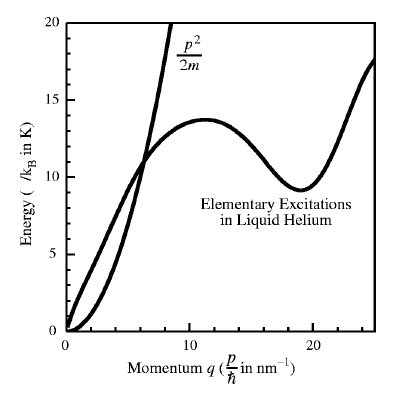
\includegraphics[width=0.5\textwidth]{FIG1.PNG} \caption{The
% dispersion curve for excitations in superfluid helium and the free
% energy of the neutron as a function of momentum transfer
% $q$~\cite{Brome2001}. The two curves cross at $q=0$ and at
% $q=q^*$, which corresponds to a neutron wavelength of 0.89~nm, oe an
% energy of
% 12~K.}  \vspace{-2.em} \label{fig:FIG1} \end{center} \end{figure}



% \item[$\bullet$] why helium? (small neutron absorption cross-section
% ) \item[$\bullet$] UCN production rate in superfluid He calculation
% (Golub77) \item[$\bullet$] Experiment shows the production rate
% matches theory (Ageron1978) and recent UCN rates
% (Zimmer2011) \item[$\bullet$] Experiment design (for example ILL
% design Baker 2003, Masuda2002, PSI source
% Anghel2009) \item[$\bullet$] Temperature of the helium source,
% (below 1K Masuda2012 )

% \item[$\bullet$] UCN storage time in superfluid helium (Golub79)
% \begin{description}



\subsubsection{Multiphonon Scattering Contribution in UCN Production in Superfluid helium~\cite{Korobkina2002,Schmidt2009}}
%So far, the UCN production was demonstrated by single phonon emission. Even though one phonon emission is the predominant process in UCN production for a monochromatic UCN beam, the
For polychromatic neutron sources, UCN can also be produced by
multiphonon processes in superfluid $^4$He. Multiphonon production of
UCN with various energy spectrum of the neutron flux has been studied
in Ref.~\cite{Korobkina2002}.  Fig.~\ref{fig:Korobkina2002} shows
the energy spectrum of neutron flux $\frac{d\phi}{dE}$ for three
sources as a function of momentum $q$ and are compared to the dynamic
scattering function $S(q,\omega=\hbar q^2/2m)$. The peak at
$q=0.7$/\AA~corresponds to the one phonon excitation by superfluid
helium. The values of $S$ above 1.2/\AA~are extrapolated. The value of
$S$ above 2/\AA~are essentially zero.  The UCN production from one
phonon and multiphonon processes have been calculated for three input
neutron spectrums: SNS ballistic guide, PULSTAR MC flux and HMI
polarized flux.  The multiphonon contribution to UCN production is
calculated by using Eqn.~(\ref{eqn:He_P_rate}) and calculating $\int
\Phi(E_1)S(k_1,\omega=\frac{\alpha k_1^2}{2}) dk_1$.  The result
showed that, for sources where helium is exposed to the total thermal
flux or at a dedicated spallation source, the multiphonon contribution
can amount to slightly more than a factor of 2 increase in the UCN
production.





\begin{figure}[h!]
\begin{center}
   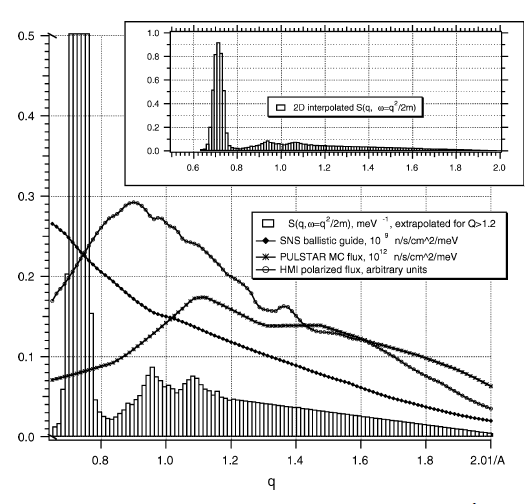
\includegraphics[width=0.7\textwidth]{Korobkina2002.PNG}
    \caption{The energy spectrum of the incident cold neutron flux
      from three sources compared to the dynamic scattering function
      $S(q,\omega=\frac{\alpha k_1^2}{2})$~/meV as a function of
      $q$~/\AA.}
%     \vspace{-2.em}
    \label{fig:Korobkina2002}
    \end{center}
\end{figure} 



%They took the energy spectrum of the neutron flux from three sources
%and extrapolated it for values of $q > 1.2$ \AA $^{-1}$ and they
%compared the results to the scattering function.

%The proposed UCN source at the North Carolina State (NC) locates a
% UCN source in the thermal column of the campus 1-MW PULSTAR reactor
% after removing the graphite. The main point of this design was the
% independence of the UCN production process to the direction of the
% incident neutrons. The proposed UCN source at the Spallation Neutron
% Source (SNS) places a superthermal UCN source on a monochromatic
% 0.89~nm beam at a guide tube. Two types of guides as ``ordinary''
% supermirror guide and ``ballistic'' guide. The ballistic guide has
% more flux at the critical 0.89~nm wavelength but less flux at
% wavelengths shorter than 0.6~nm.  The results are summarized in
% Table~\ref{tab:multiphonon}.  \begin{table} \begin{center} \begin{tabular}{|c|c|c|c|c|c|}
% \hline & NC state & SNS ord & SNS ball & HMI a.u. & Maxwell
% \\ \hline Multi-ph & 490 & 1.0 & 0.94 & 4.7 & 1.7\\ \hline Single-ph
% & 375 & 1.8 & 2.4 & 5.5 & 1.5 \\ \hline Mph/1ph & 1.4 & 0.55 & 0.4 &
% 0.85 & 1.13 \\ \hline \end{tabular} \caption{Predicted production
% rates of UCN from single and multiphonon emission from three sources
% and comparison to Maxwellian
% spectrum} \label{tab:multiphonon} \end{center} \end{table} For the
% NC state proposed UCN source, where the helium is exposed to the
% total thermal flux, the inclusion of multiphonon contribution
% increases the UCN production rate by a little more than a factor of
% 2.

%%%%%%%%%%%%%%%%%%%%%%%%%%%%%%%%%%%%%%%%%%%%%%%%%%%%%%%%%%%%%%%%%%%%%%%%%%%%%%
%% I can get rid of this part
%%%%%%%%%%%%%%%%%%%%%%%%%%%%%%%%%%%%%%%%%%%%%%%%%%%%%%%%%%%%%%%%%%%%%%%%%%%%%%
UCN production by multiphonon emission in superfluid helium under
pressure was studied in Ref.~\cite{Schmidt2009}.  The dynamic
scattering function $S(q,\omega)$ of the superfluid helium strongly
depends on pressure, leading to a pressure-dependent differential UCN
production rate. The expression for the multiphonon part of $S$
describing UCN production was derived from inelastic neutron
scattering data.  Application of pressure to superfluid helium
increases the velocity of sound, such that the dispersion curves of
the $^4$He and of the free neutron cross at shorter neutron
wavelength.

Since for neutron beams from a liquid deuterium cold source, the
differential flux density $\frac{d\Phi}{dE}$ in the range
8-9~\AA~normally increases for decreasing wavelength of the cold
neutron flux, and also since pressure increases the density of He-II,
it was expected to observe an increase in the single phonon UCN
production rate, and different multiphonon contribution with pressure
increase.  It was observed that, both the single and the multiphonon
scattering functions change with pressure. The single phonon
excitation moves to a shorter wavelength (see
Fig.~\ref{fig:Schmidt_S}) and the value for $S$ decreases. It leads to
a reduction in one-phonon UCN production.  The multiphonon excitations
increase with pressure and the peak of the scattering function $S$
moves to shorter incident-neutron wavelengths, see
Fig.~\ref{fig:Schmidt_S}. However the UCN production rate decreases
with pressure increase.  Only if the cold neutron flux at
8.3~\AA~exceeds by more than 2.5 times that at 8.9~\AA, an increase in
the UCN production rate may be expected. However, it has to be
considered that the application of pressure requires a window for UCN
extraction which causes severe UCN losses. Therefore, UCN production
in superfluid helium under pressure was concluded not to be
attractive.




\begin{figure}[h!]
\begin{center}
   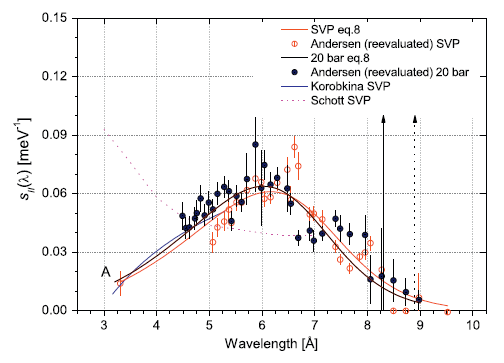
\includegraphics[width=0.7\textwidth]{Schmidt_S.PNG}
    \caption{~\cite{Schmidt2009} Multiphonon scattering function
      at SVP (Saturated Vapour Pressure) and 20bar. The extrapolation
      to short wavelength of Korobkina {\it {et
          al.}}~\cite{Korobkina2002} at SVP is linear in k,
      whereas the calculation of Schott {\it {et
          al.}}~\cite{Schott2003} is based on the static structure
      factor of the superfluid helium. The data point ($A$) is taken
      from Ref.~\cite{Fak1991}. The one-phonon peaks are indicated
      by vertical arrows: SVP (dotted line) and 20bar (solid line).  }
%     \vspace{-2.em}
    \label{fig:Schmidt_S}
    \end{center}
\end{figure} 


%%%%%%%%%%%%%%%%%%%%%%%%%%%%%%%%%%%%%%%%%%%%%%%%%%%%%%%%%%%%%%%%%%%%%%%%%%%%%%%


\subsubsection{UCN upscattering and UCN lifetime in superfluid helium~\label{sec:upscattering}}

%%%%%%%%%%%%%%%%%%%%%%%%%
%%% ADD THIS For a long UCN lifetime in superfluid helium, besides the
%%% low temperature of the converter, the $^3$He contamination must be
%%% low ($^3$He/$^4$He $\le 10^{-12}$), due to its large absorption
%%% cross-section, which requires $^4$He purification.
%%%%%%%%%%%%%%%%%%%%%%%%


Superfluid $^4$He has a zero neutron absorption cross-section and if
the converter is kept at sufficiently low temperatures (typically
$\lesssim$ 1~K), thermal upscattering of UCN is sufficiently
suppressed. This allows the produced UCN to survive in the converter
for times dominated by the wall losses of the vessel, typically
$>$100~s~\cite{Leung2016}.

The upscattering of neutrons is caused by the interactions between a
neutron at rest and excitations in superfluid helium at different
temperatures. These excitations can be categorized in three groups:
one phonon absorption, two-phonon scattering, and roton-phonon
scattering.  The total upscattering rate can be written as

\begin{equation}
\label{eqn:hE_{UCN}pscattering}
\frac{1}{\tau_{up}} =
\frac{1}{\tau_{1-ph}}+\frac{1}{\tau_{2-ph}}+\frac{1}{\tau_{rot-ph}}
\end{equation}
where,
%which are described by the following equation:
\begin{equation}
\label{eqn:1ph}
\frac{1}{\tau_{1-ph}}= A e^{-(12 K)/T}
\end{equation}
is the one phonon absorption contribution, 

\begin{equation}
\label{eqn:2ph}
\frac{1}{\tau_{2-ph}}= BT^7,
\end{equation}
is the two-phonon scattering contribution (one phonon absorbed and one
phonon emitted), and
\begin{equation}
\label{eqn:ph-rtn}
\frac{1}{\tau_{rot-ph}}= CT^{3/2}e^{-(8.6 K)/T},
\end{equation}
is the contribution from roton-phonon scattering with the absorption
of one roton followed by a phonon emission.

%The first term comes from one phonon absorption, the second term from
%two-phonon scattering where one phonon absorbed and one phonon
%emitted, and the third term from roton-phonon scattering which the
%absorption of one roton followed by a phonon emission.
The values of $A$, $B$ and $C$ are extracted from data for
temperatures up to 2.4~K~\cite{Leung2016}. The comparison between
the UCN production and upscattering rate to the theoretical
temperature dependence of these processes showed that the main
contribution is from two-phonon scattering $\frac{1}{\tau_{up}}=BT^7$
with $B=(4-16)\times 10^{-3}$~/(s K$^7$)~\cite{Leung2016}.


%The most recent study of the upscattering rates in superfluid helium
%is done by Leung {\it{et al.}}~\cite{Leung2016}.  They calculated
%the upscattering rate due to each individual excitation in a
%temperature range of 0.5~K to 2.2~K as shown in
%Fig.~\ref{fig:Leung2016}. They calculated the $A$, $B$ and $C$
%coefficients for $T \lesssim 1$~K; however, their temperature
%dependencies are weak compared to the overall sizes of the terms.
%They varied the temperature of the converter from 1.2~K to 2.4~K and
%studied the UCN production and upscattering rates. They fit data to
%the theoretical temperature dependencies of these processes and they
%determine the values of $A$, $B$ and $C$. Their analysis showed that
%they only need to include two-phonon scattering meaning
%$\frac{1}{\tau_{up}}=BT^7$ with $B=(4-16)\times 10^{-3}$~/s K$^7$.



% \begin{figure}[h!]  \begin{center}
% 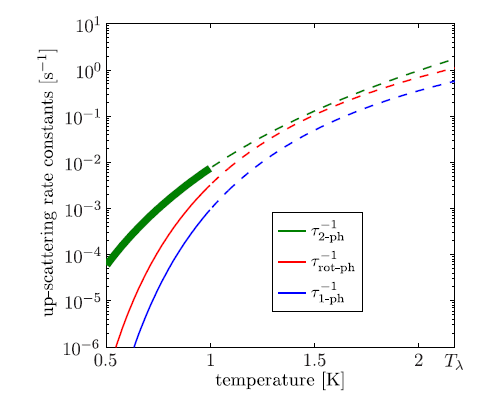
\includegraphics[width=0.5\textwidth]{Leung2016.PNG} \caption{The
% sizes of the three main processes contribution to upscattering of
% UCN by excitations in superfluid % helium from
% Eqn.~(11-14)~\cite{Leung2016}. The thickness of the
% $\tau_{2-ph}^{-1}$ line covers the rnge of values for $T < 1$~K
% owing to the different values of B ($8.8 \times
% 10^{-3}$~s$^{-1}$K$^{-7}$ at 0.6~K and $7.6
% \times10^{-3}$~s$^{-1}$K$^{-7}$ at 1.0~K). The dotted lines are used
% to indicate that the upscattering rates are only approximate for $T
% \gtrsim 1$~K due to temperature dependencies in the $A$, $B$, and
% $C$
% coefficients.}  \vspace{-2.em} \label{fig:Leung2016} \end{center} \end{figure}






%\item[$\bullet$] UCN upscattering in superfluid helium
%(Kilvington1987, Leung2016, Maris1977)


%\subsubsection{UCN lifetime in superfluid $^4$He}

\subsection{UCN production by Solid Deuterium}
Solid deuterium (sD$_2$) is a material with small absorption
cross-section, small incoherent scattering cross-section (to minimize
upscattering), and the presence of numerous phonon modes which can
inelastically scatter neutrons down to UCN energies.
%In solid D$_2$ the phonon excitations are present in the coherent
%part of the scattering, whereas the incoherent part is determined by
%rotational transitions and also by incoherent phonon scattering.
A converter based on sD$_2$ should be operated at temperatures below
10~K in order to avoid subsequent upscattering of UCN by phonons
within solid deuterium.
% The employment of solid deuterium at 10~K increases UCN yield by 10
% times compared with the UCN yield from liquid
% deuterium~\cite{Serebrov2000}.
 
Solid deuterium has an almost perfect hcp crystal structure, when
prepared under suitable conditions (low pressure and $T >$~5~K). The
D$_2$ molecule has internal rotational modes which are described by
the rotational quantum number $J$. The rotational excitations give
rise to additional modes in the solid deuterium. %In the solid phase,
$J$ is still a good quantum number.  Deuterium in the states with even
$J$ is called ortho-deuterium (o-D$_2$) whereas deuterium in the
states with odd $J$ is called para-deuterium (p-D$_2$). An increase of
the concentration of the p-D$_2$ molecules leads to a larger neutron
upscattering rate.
%The self-conversion between these two species in the solid phase is
%extremely slow compared with the time scale of the experiment and
%therefore, using a para- t ortho- converter is essential.  At low
%temperatures ($T\sim$~6~K), about 99.999\% of the deuterium molecules
%are in the ortho state, when thermal equilibrium is reached. At room
%temperature, D$_2$ has an ortho concentration of 66.7\%.
Theoretically and experimentally it has been shown that sD$_2$ at
sufficiently low temperatures (around 5K) with high enough purity and
with high ortho concentration can be used to produce a high density
UCN~\cite{Atchison2005}.

% The common principle is to expose sD$_2$ to a high flux of cold
% neutrons in order to produce UCN. It was shown that, using a pulsed
% neutron beam to produce UCN resulted in densities 4-5 orders of
% magnitude greater than the reactor-based UCN
% sources~\cite{Pokotilovski1995}.  The UCN production rate here
% is a factor of 30 larger as compared to superfluid helium, since the
% phonon spectrum has a much higher phase space density for the
% downscattering of cold neutrons~\cite{Golub83}. The UCN density
% in such sources is limited by nuclear absorption in the converter
% medium, and UCN lifetime.  Below 5K, upscattering in sD$_2$ is less
% important than absorption~\cite{Liu2000}.





\subsubsection{UCN Production Cross-Section and UCN Production Rate in Solid Deuterium~\cite{ucnbook,Frei2010,Frei2009}}

The formula for the UCN production in solid deuterium is very similar
to that of the superfluid helium shown in Eqn.~(\ref{UCN_production})
with replacing $^4$He atomic density $N_{\text{He}}$ with molecular density
of solid deuterium $N_{D_2}$ and noting that in sD$_2$ the neutron
scattering cross-section may be written as a sum of coherent and
incoherent contributions:

\begin{equation}
\label{eqn:dsigma}
\frac{d\sigma}{d\omega}=\left[ \frac{k_2}{k_1} 
b_{\text{coh}}^2 S_{\text{coh}} (q,\omega) + \frac{k_2}{k_1} b_{\text{inc}}^2 S_{\text{inc}}(q,\omega) \right]
 d\Omega.
\end{equation}
In Ref.~\cite{Frei2010} the UCN production cross-section $\sigma$
was determined by two ways. One way is the determination of the
quasi-particle (phonons and rotational excitations of the D$_2$
molecule) density of states $G_1(E)$ (incoherent approximation) from
the measured neutron cross-section $\frac{d\sigma}{d\omega}$ and the
other method is the direct integration of the dynamical neutron
cross-section $\frac{d\sigma}{d\omega}$ ($\hbar=1$) in the kinematical
region along the free-neutron dispersion parabola.

\paragraph{UCN production cross-section: Incoherent approximation.}
With the knowledge of the quasi-particle density of states $G_1(E)$,
it is possible to calculate the dynamical neutron cross-section
$\frac{d\sigma}{d\omega}$ (averaged over the scattering angle, thus
$q$). Vice versa it is also possible to extract $G_1(E)$ from a
measured dynamical neutron cross-section~\cite{Turchin}.  If
$G_1(E)$ is known, it is possible to calculate one-phonon and
multiphonon contributions to the neutron cross-section
$\frac{d\sigma}{d\omega}$.
% In the incoherent
% approximation \begin{equation} \label{eqn:G} \frac{d\sigma}{d\omega}=\frac{k_2}{k_1}[b_{eff}(q)]^2 \frac{\hbar
% q^2}{2m}\frac{G(\omega)}{\omega} \left[ n(\omega)+1 \right]
% e^{-2W(q)} \end{equation} where $G(\omega)$ is the generalized
% density of states (GDOS). With the measured inelastic neutron
% cross-section and Eqn.~(\ref{eqn:G}), it is possible to determine
% the GDOS.  $G(\omega)$ comprises the complete phonon excitations of
% sD$_2$ as well as rotational transitions of individual D$_2$
% molecules. Furthermore, multiphonon excitations of the phonon system
% of sD$_2$ should appear in the GDOS as they are not corrected for in
% Eqn.~(\ref{eqn:G}).  GDOS for differently prepared D$_2$ crystals at
% the same o-D$_2$ concentration is measured for o-D$_2$ 66.7\% and
% 95\%~\cite{Frei2009}. The result did not show variations beyond
% statistical effects.  The main difference between the GDOS for
% different o-D$_2$ concentrations was the strength of the rotational
% transition $J=0\rightarrow 1$. Increasing the o-D$_2$ concentration
% enhances this transition.


% The generalized density of states (GDOS) $G(\omega)$ is measured to
% ultimately calculate dynamical neutron cross-section (incoherent
% approximation). $G(\omega)$ comprises the complete phonon
% excitations of sD$_2$ as well as rotational transitions of
% individual D$_2$ molecules. Furthermore, multiphonon excitations of
% the phonon system of sD$_2$ should appear in the GDOS.  GDOS for
% differently prepared D$_2$ crystals at the same o-D$_2$
% concentration was measured for o-D$_2$ 66.7\% and
% 95\%~\cite{Frei2009}. The result did not show variations beyond
% statistical effects.  The main difference between the GDOS for
% different o-D$_2$ concentrations was the strength of the rotational
% transition $J=0\rightarrow 1$.  Increasing the o-D$_2$ concentration
% enhances this transition.
% Fig.~\ref{fig:Frei2010fig}~\cite{Frei2010} shows two examples of
% neutron scattering data for two different concentrations of o-D$_2$
% molecules as a function of energy transfer $E=E_i-E_f$.  The density
% of state (DOS) $G_1$ can be extracted from GDOS data, and it leads
% to the calculation of $d\sigma/dE$. Studies showed
% that~\cite{Frei2010}, an increase in the concentration of the
% p-D$_2$ molecules leads to a larger neutron upscattering.  This
% upscattering has serious implications to the upscattering of UCN in
% the sD$_2$ converter material, and reduces the achievable density of
% UCN in sD$_2$.  It is also shown that, the elastic cross-section
% ($E=$0~meV) of sD$_2$ is quite large.  The one-particle excitation
% on the dynamic neutron scattering cross-section is above E$=$10~meV,
% two-particle contributions is above E$\sim$5~meV, and three particle
% excitations above E$=$12~meV~\cite{Frei2009}.
The method for the determination of $G_1(E)$ from the measured neutron
scattering data in solid deuterium is studied in
Ref.~\cite{Frei2009}.  In the determination of $G_1(E)$,
contributions of higher order multiphonons to $\frac{d\sigma}{dE}$ are
incorporated.

In the case of UCN production the energy transfer of the downscattered
neutron $E=E_1-E_{\text{UCN}}$ is approximately equal to the initial
neutron energy $E_1$ ($E_{\text{UCN}} \ll E_1, E_{\text{UCN}}$: UCN
energy). The total cross-section for UCN production can be calculated
by

\begin{equation}
\sigma_{\text{UCN}}({E_1})=\int_0 ^{E_{\text{UCN}}^{max}} \frac{d\sigma (E_1)}{dE} dE_{\text{UCN}}.
\end{equation}

The calculated cross-section is shown in
Fig.~\ref{fig:Frei2010_sigma_G1} is in agreement with data on UCN
production using a cold neutron beam ($E_1 \sim 1.4$~meV to 20~meV).
Here the one-quasi-particle and two-quasi-particle excitations are
included in the calculations.  The UCN production cross-section is
mainly determined by one-quasi-particle excitation for energies below
15~meV. The two-quasi-particle contribution is non-negligible in the
region of 5-25~meV.

The application of the incoherent approximation in the case of sD$_2$
has certainly to be questioned since the sD$_2$ crystal scatters
neutrons more coherently than incoherently.

\begin{figure}[h!]
\begin{center}
   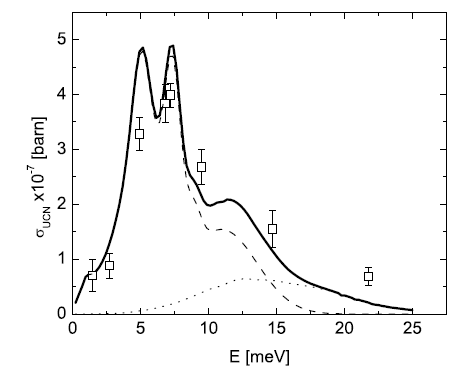
\includegraphics[width=0.5\textwidth]{Frei2010_sigma_G1.PNG} \caption{UCN
    production cross-section of sD$_2$ with 98\% ortho
    concentration. UCN energy range 0-150~neV inside the solid
    D$_2$. Solid line: cross-section calculated in incoherent
    approximation. Dashed line: one-quasi-particle
    contribution. Dotted line: two-quasi-particle
    contribution. $\square$: data from measurements at
    PSI~\cite{Atchison2007}.  }
%     \vspace{-2.em}
    \label{fig:Frei2010_sigma_G1}
    \end{center}
\end{figure} 




\paragraph{UCN production cross-section: Direct determination.}
The easiest way of determining the cross-section for UCN production is
the use of the dynamical scattering function $S(q,\omega)$ in the
($q,\omega$)-phase space along the free-neutron parabola, as shown
schematically in Fig.~\ref{fig:sD2_S}.

This method allows the incorporation of all the coherent and
incoherent contributions to the UCN production cross-section. Possible
coherent contributions, which cannot be treated exactly with the
incoherent approximation, appear directly in the deduced
cross-section. Therefore, this method is superior in principle to the
result obtained by the incoherent approximation.

\begin{figure}[h!]
\begin{center}
   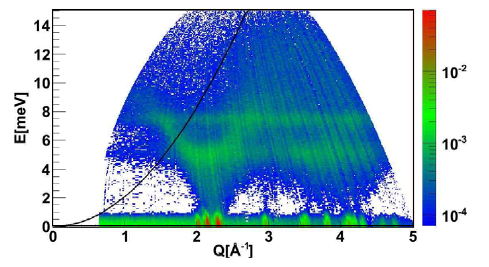
\includegraphics[width=0.7\textwidth]{sD2_S.PNG} \caption{\cite{Frei2010}
    $S(q,\omega)$ ($q=Q ,\omega=E$) (arb. units) of 95.2\% solid
    o-D$_2$ at $T=4$~K. Data from IN4 measurements. Black parabola:
    dispersion of the free neutron. }
%     \vspace{-2.em}
    \label{fig:sD2_S}
    \end{center}
\end{figure} 



The UCN production cross-section can be determined by
\begin{equation}
\sigma_{\text{UCN}}(E_1)=\frac{\sigma_1}{k_1} S(k_1, E_1) \frac{2}{3} k_{\text{UCN}}^{max} \; E_{\text{UCN}}^{max} 
\end{equation}
where $E_1$ is the energy of the incoming neutrons in the
downscattering process, $\sigma_1$ is a constant and
$k_{\text{UCN}}^{max}$ and $E_{\text{UCN}}^{max} $ are the upper
limits for the UCN momentum and energy.  In order to obtain absolute
cross-sections, $S(q,\omega)$ has to be calibrated to absolute values.
The result of this calibration and the determination of the UCN
production cross-section as a function of the energy of the incoming
neutrons, and a comparison with the measurements of this cross-section
is shown in Fig.~\ref{fig:Frei2010fig2}. This plot also contains the
data, which were obtained with higher incoming-neutron energy
($E_1=67$~meV).


\begin{figure}[h!]
\begin{center}
   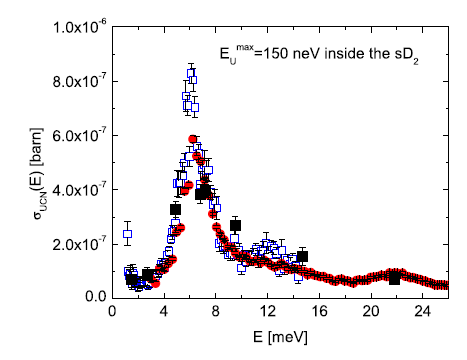
\includegraphics[width=0.5\textwidth]{Frei2010_sigma.PNG} \caption{\cite{Frei2010}
    UCN production cross-section solid o-D$_2$ of
    95.2\%~\cite{Frei2010}. A UCN energy range of 0-150~neV inside
    the solid D$_2$ is assumed. Sample: fast frozen solid deuterium
    ($T=4$~K); data from IN4 measurements. Blue $\square$:
    $E_0=17.2$~meV. Red filled $\bigcirc$: $E_0=67$~meV,
    $\blacksquare$: direct UCN production data from measurements at
    PSI~\cite{Atchison2007}.  }
%     \vspace{-2.em}
    \label{fig:Frei2010fig2}
    \end{center}
\end{figure} 

The comparison of the calculated UCN production cross-section,
extracted from the incoherent approximation and parabola method, shows
(see Fig.~\ref{fig:Frei2010_sigma_G1} and Fig.~\ref{fig:Frei2010fig2})
a discrepancy in the region of $E\sim6$~meV.  The cross-section
determined by the parabola method shows a pronounced maximum in the
region of $E\sim6$~meV as compared to the incoherent approximation
result. This peak corresponds to the coherent phonon contribution to
the UCN production cross-section. The double-peak structure in the UCN
production cross-section by the incoherent approximation is not
present in Fig.~\ref{fig:Frei2010fig2} and cannot be reproduced by the
measured data shown in Figs.~\ref{fig:Frei2010_sigma_G1}
and \ref{fig:Frei2010fig2}.  This means, a new experiment at a more
intense cold neutron beam with a better energy resolution would be
desirable to study this effect further.

In Fig.~\ref{fig:sD2_S}, the parabola of the free neutron crosses the
acoustical phonon dispersion curve at $E \sim 6$~meV. At this point,
the UCN production cross-section is predominantly determined by
coherent scattering.  This can explain a deviation from the production
cross-section in incoherent approximation. Nevertheless the general
agreement of the incoherent approximation with the PSI data is
remarkable (as shown in Fig.~\ref{fig:Frei2010_sigma_G1}).


%The coherent phonon contribution to the UCN production cross-section
%at $E \simeq 5$~meV, which is clearly seen in
%Fig.~\ref{fig:Frei2010fig2}, is a major downscattering channel for
%UCN production.

The result for the calculated UCN production rate in solid o-D$_2$,
exposed to a Maxwellian shaped neutron flux for different effective
neutron temperatures is shown in
Fig.~\ref{fig:sD2_production_rate}. The main conclusion from these
results was the new understanding of possible higher energetic loss
channels (one-quasi-particle and two-quasi-particle) in solid
deuterium for the downscattering of cold neutrons in the conversion
process to UCN. The best value for the effective neutron temperature
is in the region of $T_n \sim 40$~K which is larger than what was
previously expected ($T_n \sim 30$~K~\cite{Yu1986}).



\begin{figure}[h!]
\begin{center}
   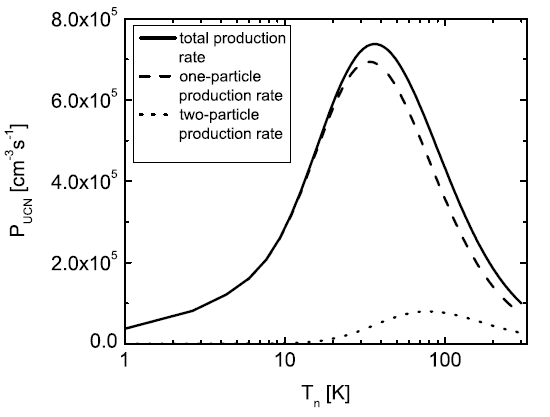
\includegraphics[width=0.5\textwidth]{Frei2010_P.PNG} \caption{\cite{Frei2010}
    Calculated UCN production rate of sD$_2$ with 98\% ortho
    concentration for different Maxwellian neutron spectra with
    effective neutron temperature $T_n$. UCN energy range:0-150~neV
    inside the sD$_2$. Neutron capture flux $10^{14}$~/cm$^2$s. Solid
    line: total production rate (one- and two- particle
    excitations). Dashed line: one-particle production rate. Dotted
    line: two-particle production rate.}
%     \vspace{-2.em}
    \label{fig:sD2_production_rate}
    \end{center}
\end{figure} 





% \subsubsection{Neutron scattering study} Neutron scattering is an
% excellent tool to investigate the phonon system and the rotational
% transitions of D$_2$ molecules in sD$_2$.  The dynamics of sD$_2$ is
% studied by means of inelastic scattering (coherent and incoherent)
% of thermal and cold neutrons at different temperatures and
% para-ortho ratios~\cite{Frei2009}.  Scattering of neutrons where
% a rotational transition ($ J \rightarrow J^{\prime}$ and $J \neq
% J^{\prime}$) is involved leads to an incoherent response of the
% system. The phonon excitations are present in the coherent part of
% the scattering, whereas the incoherent part is determined by
% rotational transitions and also by incoherent phonon scattering.


% The generalized density of states (GDOS) $G(\omega)$ is measured to
% ultimately calculate dynamical neutron cross-section (incoherent
% approximation). $G(\omega)$ comprises the complete phonon
% excitations of sD$_2$ as well as rotational transitions of
% individual D$_2$ molecules. Furthermore, multiphonon excitations of
% the phonon system of sD$_2$ should appear in the GDOS.  GDOS for
% differently prepared D$_2$ crystals at the same o-D$_2$
% concentration was measured for o-D$_2$ 66.7\% and
% 95\%~\cite{Frei2009}. The result did not show variations beyond
% statistical effects.  The main difference between the GDOS for
% different o-D$_2$ concentrations was the strength of the rotational
% transition $J=0\rightarrow 1$.  Increasing the o-D$_2$ concentration
% enhances this transition.
% Fig.~\ref{fig:Frei2010fig}~\cite{Frei2010} shows two examples of
% neutron scattering data for two different concentrations of o-D$_2$
% molecules as a function of energy transfer $E=E_i-E_f$.  The density
% of state (DOS) $G_1$ can be extracted from GDOS data, and it leads
% to the calculation of $d\sigma/dE$. Studies showed
% that~\cite{Frei2010}, an increase in the concentration of the
% p-D$_2$ molecules leads to a larger neutron upscattering.  This
% upscattering has serious implications to the upscattering of UCN in
% the sD$_2$ converter material, and reduces the achievable density of
% UCN in sD$_2$.  It is also shown that, the elastic cross-section
% ($E=$0~meV) of sD$_2$ is quite large.  The one-particle excitation
% on the dynamic neutron scattering cross-section is above E$=$10~meV,
% two-particle contributions is above E$\sim$5~meV, and three particle
% excitations above E$=$12~meV~\cite{Frei2009}.



% \begin{figure}[h!]  \begin{center} 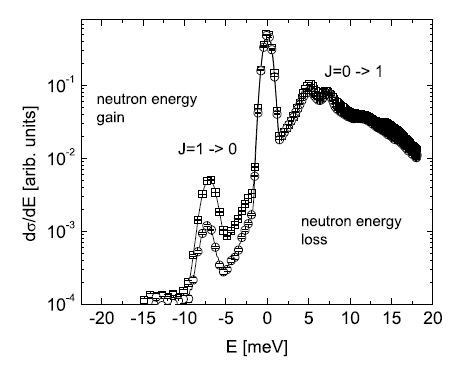
\includegraphics[width=0.5\textwidth]{FREI2010.PNG} \caption{An
%    example of the dynamical neutron cross-section of solid deuterium
%    at T$=7$~K. Comparison of two ortho concentrations c$_0$=66.7\%
%    ($\square$) and c$_0$=98\% ($\bigcirc$). Data from TOFTOF
%    measurements at the FRM II. Initial energy of the thermal
%    neutrons is E$_0=$20.4~meV~\cite{Frei2010}. }
%%     \vspace{-2.em}
%     \label{fig:Frei2010fig}
%     \end{center}
% \end{figure} 





\subsubsection{UCN upscattering and UCN lifetime in sD$_2$~\cite{Liu2000,Morris2002}}


The different molecular species ortho-D$_2$ and para-D$_2$ have
significantly different UCN-phonon annihilation
cross-sections~\cite{Liu2000}. The presence of even small
concentrations of para-D$_2$ can dominate the upscattering rate which
gives rise to reduced UCN lifetimes in the solid and orders of
magnitude reduction in the achievable UCN density.  In a D$_2$ solid,
the populations of ortho and para states are typically determined by
the ortho/para population of the gas phase before the D$_2$ is frozen
into solid.  After cooling down the D$_2$ to the solid phase
($T \sim$~6~K), it normally takes months to reach the equilibrium of
99.999\% o-D$_2$.
 %The selfconversion between these two species in the solid phase into
 %a thermal Boltzman distribution is extremely slow compared with the
 %time scale of experiment.  Since the elimination of para-D$_2$ is
necessary to achieve UCN lifetimes comparable to the nuclear
absorption time in solid deuterium, using a para-D$_2$ to ortho-D$_2$
converter is crucial.


\begin{figure}[h!]
\begin{center}
   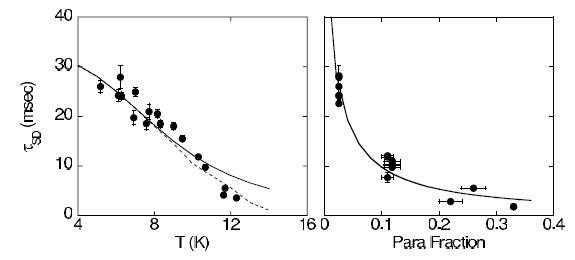
\includegraphics[width=0.6\textwidth]{Morris2002.PNG} \caption{\cite{Morris2002}
    Left- Data points are measured sD$_2$ lifetimes as a function of
    temperature, with the para-fraction fixed at 2.5\%. Only the
    statistical errors are shown. Solid lines show the predicted
    temperature dependence. The dashed line is the predicted effect of
    departure from the solid lifetime model due to upscatter from
    D$_2$ gas in the guide. Right- sD$_2$ lifetimes as a function of
    para-fraction for all of the data taken below 6~K. The solid line
    is the model prediction of the para-fraction dependence at an
    average temperature of 5.6~K.  }
%     \vspace{-2.em}
    \label{fig:Morris2002}
    \end{center}
\end{figure} 



%\subsubsection{UCN lifetime in sD$_2$}
The lifetime of the UCN in sD$_2$ is limited by factors such as
 upscattering from phonons in the solid, upscattering from p-D$_2$
 contamination and absorption inside the vessel.  Reducing the time
 UCN spend inside the sD$_2$ can reduce the average absorption
 rate. This led to the proposal of a thin-film source where a thin
 layer of solid D$_2$ coats the inside of a storage bottle that is
 embedded in a cold neutron flux~\cite{Golub83}. The possibility
 of a smaller source volume combined with the higher operating
 temperature of the thin film source offers significant technical
 simplification.

The UCN lifetime in the solid deuterium as a function of temperature
and para/ortho fractions has been measured~\cite{Morris2002}. The
total loss rate can be written as

\begin{equation}
\label{eqn:SD_lifetime}
\frac{1}{\tau_{SD}}=\frac{1}{\tau_{phonon}}+\frac{1}{\tau_{para}}+\frac{1}{\tau_{Dabs}}+ \frac{1}{\tau_{Habs}}
\end{equation}
where, $\frac{1}{\tau_{phonon}}$ is the upscattering rate from phonons
in SD$_2$, $\frac{1}{\tau_{para}}$ is the upscattering rate from para
deuterium molecules in the solid, $\frac{1}{\tau_{Dabs}}$ is the
upscattering rate from the absorption on deuterium and
$\frac{1}{\tau_{Habs}}$ is the upscattering rate from the absorption
on the hydrogen impurities in the solid. The results for UCN lifetimes
$\tau_{SD}$ in sD$_2$ as a function of the sD$_2$ temperature and
para/ortho fractions are shown in Fig.~\ref{fig:Morris2002}. The
difference between the solid and dashed line demonstrates the need to
include the effect of deuterium vapor in the guide on the lifetime at
higher temperatures. With this correction, the measured lifetimes
agree well with theoretical predictions of the upscattering rate.





%They demonstrated the necessity of including the effect of deuterium
%vapor in the UCN guide on the lifetime at higher temperatures to
%achieve an agreement with the theoretical predictions of UCN
%lifetime.  The storage time for UCN in the presence of an exit hole
%is $1/\tau_{tot}=1/\tau_{h}+1/\tau_0$ where $1/\tau_{h}$ is the loss
%rate of UCN through exit hole and $\tau_0$ is the storage time in the
%absence of the hole.  (????? not convincing for the next line!!!!! I
%need to add something here.)

%
%The temperature should be low enough so that the absorption in the film is greater than the upscattering rate.

%\item[$\bullet$] why deuterium? (weak neutron absorption
%cross-section from UCN book and Atchison2005,
%Altarev1980) \item[$\bullet$] UCN production with solid Deuterium
%(Frei2007 and Lauer2013 for Mainz and Morris2002 and Saunders2013 for
%Los Alamos) \item[$\bullet$] upscattering rates
%(Liu2000) \item[$\bullet$] thin film sources?? ( in the UCN
%book) \item[$\bullet$] production of UCN at pulsed neutron source
%(Pokotilovski1995)
\subsection{Comparison between sD$_2$ and superfluid helium sources}

The main differences between sD$_2$ and superfluid helium sources are
the UCN lifetime and the UCN production rate. While UCN can stay in
superfluid helium until it $\beta$-decays, UCN in solid deuterium are
absorbed by the deuteron in 150~ms after they are produced.  Once a
superfluid helium source is cooled down to temperatures below 0.75~K,
the upscattering rate is suppressed to a level comparable to neutron
$\beta$-decay.  Solid deuterium has a production rate two orders of
magnitude greater than superfluid helium. Therefore, solid deuterium
sources output higher UCN current compared to superfluid helium
sources. However, the limiting production time in superfluid helium is
four orders of magnitude longer than sD$_2$. Thus, even with a smaller
UCN production rate, superfluid $^4$He can in principle achieve a UCN
density larger than that of solid deuterium.  The superthermal
enhancement in solid deuterium is limited by the large nuclear
absorption loss, and thus further cooling below 5~K will not
significantly enhance the UCN yield.

%Both types of sources use quantum excitations in the converter medium
%to create the UCN; these are phonons in the case of sD$_2$ and
%phonons and rotons in the case of superfluid $^4$He. Since $^4$He
%does not capture neutrons and has a small upscattering probability
%for UCN, the superfluid $^4$He source can be operated at lower
%currents for longer times, allowing a large density of neutrons to
%accumulate. Storage times of hundreds of seconds are
%achievable. Solid deuterium sources, on the other hand, must pulse
%the beam, then quickly isolate any UCN produced from the sD$_2$,
%usually with a valve directly above the deuterium, because a UCN in
%sD$_2$ will only survive for tens of milliseconds.  The TRIUMF's
%technology is therefore complementary to spallation sD$_2$ projects.






%While the thin film source produces lower UCN densities than the
%helium-based source, the ability of this source to operate with
%shorter storage times without further loss of UCN density will allow
%either a large beam area or a smaller source volume or some
%combination.
\subsection{Other UCN Sources~\cite{Salvat2013,Atchison2009,Liu_thesis}}

Superthermal UCN sources may be compared by

\begin{equation}
\sigma_s / \sigma_a
\end{equation}

where $\sigma_s$ is the elastic scattering cross-section and
$\sigma_a$ is the absorption cross-section. At low energies ($<$~1~eV)
$\sigma_a \sim 1/v$ where $v$ is the speed of the neutrons. This
means, the absorption cross-section is much larger at lower energies.
Table~\ref{tab:other_sources} shows a list of possible superthermal
UCN sources~\cite{Liu_thesis}. The values of $\sigma_a$ are for
thermal neutrons.


\begin{table}
\begin{center}
\begin{tabular}{|l|l|l|}
\hline
Isotope & $\sigma_a$(barns) & $\sigma_s / \sigma_a$  \\
\hline
$^2$D & 0.000519 & 1.47 $\times 10^4$ \\
\hline
$^4$He & 0 & $\infty$ \\
\hline
$^{15}$N & 0.000024 & 2.1 $\times 10^5$ \\
\hline
$^{16}$O & 0.00010 & 2.2 $\times 10^4$ \\
\hline
$^{208}$Pb & 0.00049 &  2.38 $\times 10^4$\\
\hline
\end{tabular}
\end{center}
\caption{Candidates for a superthermal source\label{tab:other_sources}}
\end{table}

Solid $\alpha - ^{15}$N$_2$ is a potential alternative to
deuterium~\cite{Salvat2013}. its absoption cross-section is only
5\% of that of D$_2$, and it has a negligible incoherent scattering
cross-section. Additionally, rotation of the N$_2$ molecules in the
lattice is inhibited due to the anisotropy of the N$_2$
inter-molecular potential. This leads to dispersive modes for the
rotational degrees of freedom (librons) which provide additional
channels for neutron downscattering and eliminates the rotational
incoherent upscattering. Measurements~\cite{Salvat2013} show that
the production cross-section peaks near 6~meV and the optimal incident
cold neutron temperature is 40~K. It was found that the variation in
the cross-section is no more than 18\% in the range from 5 to 25~K
(increasing slightly with increasing temperature).  The measured
cross-section was found to be somewhat lower than that of D$_2$ and
O$_2$.
%However, it has a longer mean free path compared to deuterium.
A nitrogen-based source may benefit from operating at lower
temperatures, if the upscattering cross-section can be further reduced
at lower temperatures ($\sim$1~K)~\cite{Salvat2013}.


$^{208}$Pb and solid deuterium have similar nuclear absorption
cross-sections. The natural solid form of $^{208}$Pb would avoid the
difficulties of growing cryogenic solids such as deuterium and
oxygen. However, its heavy mass prevents the neutron momentum transfer
to the solid phonon field. The heavy mass reduces the phonon creation
cross-section by $1/M$. As a result one would expect its UCN yield to
be two orders of magnitude less than solid deuterium.

As other options, the properties of the new candidate converter
materials including solid heavy methane (CD$_4$) and solid oxygen
(O$_2$) have been investigated in the temperature range 8~K to room
temperature by measuring the production of UCN from a cold neutron
beam and the cold neutron transmission through the converter
materials~\cite{Atchison2009}. The liquid O$_2$, D$_2$ and CD$_4$
have similar neutron scattering cross-sections.

$^4$He and D$_2$ are still the best commonly pursued options, although
there is a chance that other materials could lead to a breakthrough.
% \item[$\bullet$] Investigationofsolid D$_2$, O$_2$ and CD$_4$ for
% UCN production (Atchison2009) \item[$\bullet$] Investigating solid
% $\alpha$-$^{15}$N$_2$ as a new source of ultra-cold neutrons
% (Salvat2013) \item[$\bullet$] solid $\alpha$-oxygen (Gutsmiedl2011,
% Liu thesis)



% \subsubsection{UCN Production Rate with Single Phonon scattering in
% Superfluid helium} Golub and Pendlebury 1975 and 1977

% \subsubsection{Multiphonon Scattering Contribution in UCN Production in Superfluid helium}
% Korobkina {\it{et al.}} and Schott {\it{et al.}}

% \subsubsection{Neutron Upscattering Rate in Superfluid helium}
% Leung {\it{et al.}} and Maris {\it{et al.}}


% \subsubsection{UCN Production Rate with SD$_2$ converter}



% \subsubsection{UCN Upscattering Rate in SD$_2$}
% Liu {\it{et al.}}



% \section{UCN Extraction}
% Cut if possible


\section{Current Status of UCN sources Worldwide}
\subsection {It needs to be modified}
New UCN sources using superthermal technology are under development at
various laboratories across the world.  Neutrons are produced by two
methods: proton-induced spallation off a heavy nuclear target
({\it{e.g}}.~tungsten), and fission where neutrons are produced by a nuclear
reactor. Table~\ref{tab:full_ucn_sources}~\cite{Jeff_dnp} shows a
list of the present and future UCN sources worldwide.



\begin{table}[h!]
\begin{center}
\begin{tabular}{|l|l|l|l|}
\hline
Name & Source Type & Technology & Status \\
  \hline
  \hline
ILL  & Turbine & Reactor, CN beam & Running
%39 & few s 
\\
\hline
%J-PARC & Doppler SHifter & Spallation & Running
%\\
%\hline
ILL SUN-2 & LHe & Reactor, CN beam & Running 
%$\sim$15 peak (60~s,30~L) & 200(4~L, Fomblin grease, 80~neV)
\\
\hline
ILL SuperSUN & LHe & Reactor, CN beam & Future
%$\sim$150 peak (60~s, 30~L)& 800 %(12~L, 230~neV magnetic trap)
\\
\hline
%RCNP/KEK & LHe & Spallation & 26 & 81 (Ni) \\
%\hline
RCNP/TRIUMF/KEK & LHe & Spallation & Installing/Future
%600 polarized & 100 (NiP)
\\
\hline
PNPI Gatchina & LHe & Reactor & Future
%12000 & 10 (from He at 1.2~K)
\\
\hline
%ILL Turbine & sD$_2$ & Turbine & 39 & Few s \\
%\hline
LANL & sD$_2$ & Spallation & Running/Upgrading
%$\sim$25 polarized & 40 
\\
\hline
PSI & sD$_2$ & Spallation & Running
%Peak$\sim$23 & $\sim$90~s
\\
\hline
Mainz & sD$_2$ & Reactor & Running
%10 & Few s
\\
\hline
FRM II, Germany & sD$_2$ & Reactor & Future
%$\sim$5000 & Few s
\\
\hline
NCSU PULSTAR & sD$_2$ & Reactor & Installing
%$>$30 & Few s
  \\
  \hline
  SNS, Oakridge & LHe & Spallation & Future
  \\
  \hline
  J-PARC & Doppler Shifter & CN beam & Running
  \\
  \hline
\end{tabular}
\end{center}
\caption{Existing and future UCN sources worldwide. The existing or
  proposed sources at the following sites is listed: Institut
  Laue-Langevin~(ILL) in France, Reasearch Center for Nuclear
  Physics~(RCNP) in Japan, KEK and J-PARC in Japan, TRIUMF in Canada,
  Petersburg Nuclear Physics Institute~(PNPI) in Russia, Los Alamos
  National Lab~(LANL), PULSTAR and SNS in the US, Mainz and FRM II in
  Germany. }
\label{tab:full_ucn_sources}
\end{table}






Reactor sources place the moderators close to the reactor core~(FRM~II
and Gatchina~\cite{Serebrov_ascona}) or use existing CN beam lines
(ILL~\cite{Piegsa2014}). At FRM~II, the sD$_2$ will be placed
around a solid hydrogen cold-moderator close to the fuel element. The
Gatchina superfluid $^4$He source will be placed inside their thermal
column, using immense pumping power to cool the converter to 1.1~K,
making rapid extraction necessary due to increased UCN upscattering at
this temperature.

The SuperSUN and SUN-2 experiments are the logical extensions of the
early superthermal source geometry at ILL.  A novel feature of the
SuperSUN experiment at ILL~\cite{Zimmer2015} is a magnetic
multipole reflector for a drastic enhancement of the UCN density with
respect to an existing prototype superfluid helium UCN source
installed in a cold neutron beam. A multipole magnet can lead to a
large gain in the saturated density of low-field-seeking UCNs because
the presence of the field reduces the number of neutrons hitting the
material walls and reduces the energy and wall collision rate of those
that do. In addition, it acts as a source-intrinsic UCN polarizer
without need to polarize the incident beam and hence avoiding
associated losses.
%This concept will lead to a drastic improvement of previous UCN
%storage time constants and hence provide a polarised UCN density
%beyond 1000 per cm$^3$.

The Los Alamos solid deuterium source~\cite{Ito_ascona} uses a
proton beam of 900~MeV and a W target to produce neutrons. The
neutrons get cooled down in a polyethylene cold moderator. The new
design includes a flapper valve to isolate the neutrons from the
sD$_2$ after the proton beam pulse.

The PSI UCN source~\cite{Ries_ascona} uses a 600~MeV proton beam
to hit a Pb/Zr target for neutron production. They use a 30~L volume
of sD$_2$ at 5~K as moderator and converter to produce UCN. This
volume is surrounded by D$_2$O thermal moderator. They also use a
flapper valve for UCN extraction between the proton beam pulses to
limit the losses. The UCN production has been running since 2012 with
an on-going EDM experiment, with a peak density of 23~UCN/cm$^3$.

The Mainz UCN source~\cite{Karch2014} is the only source that
operates at a low power university reactor and is the newest
production source. The solid deuterium converter with a volume of V =
160 cm$^3$, which is exposed to a thermal neutron fluence of 4.5
$\times 10^{13}$ n/cm$^2$, delivers up to 240000 UCN ($v \leq$ 6~m/s)
per pulse outside the biological shield at the experimental area.  UCN
densities of $\approx$ 10/ cm$^3$ are obtained in stainless-steel
bottles of V $\approx$ 10~L. Their pulsed operation permits the
production of high densities for storage experiments.


At the SNS UCN source, the 8.9~$\AA$ cold neutrons are selected using
a monochromator, and are transported with neutron guides to two cells
made out of acrylic~(ultraviolet transmitting) and separated by a high
voltage electrode.  The neutrons entering the cell are
polarized. Within the cell, the cold neutrons become ultra-cold
neutrons via $^4$He single-phonon process~\cite{kolarkar2010}.


The UCN source at J-PARC is a doppler-shifter type of pulsed UCN
source~\cite{Imajo2015}. Very cold neutrons~(VCNs) with 136~m/s
velocity in a neutron beam supplied by a pulsed neutron source are
decelerated by reflection on a $m=10$ wide-band multilayer mirror,
yielding pulsed UCN. The mirror is fixed to the tip of a 2,000~rpm
rotating arm moving with 68~m/s velocity in the same direction as the
VCN. The repetition frequency of the pulsed UCN is 8.33~Hz and the
time width of the pulse at production is 4.4~ms. In order to increase
the UCN flux, a supermirror guide, wide-band monochromatic mirrors,
focus guides, and a UCN extraction guide have been newly installed or
improved. This source will be used to search for the nEDM.


The UCN source at TRIUMF will use a W target to produce spallation
neutrons from a 500~MeV proton beam on site. The cold neutrons will be
converted to UCN in superfluid helium.  this source is projected to
compete with the capabilities of the best planned future UCN
sources. If TRIUMF's estimated UCN density of 680 UCN cm$^{-3}$ is
achieved, it will be a new world record. Other sources and nEDM
experiments aim at similar goals of hundreds to thousands of UCN
cm$^{-3}$ in the measurement volume. However, to date, superthermal
sources have not produced considerably more UCN than the ILL turbine
source.


% Russ said: "This paragraph could be part of the conclusion.  The
% first paragraph should summarize what a superthermal source is and
% the main differences between He and sD2.  Then this paragraph.
 


%The neutrons are neutral particles, subjected to all fundamental
%forces which helps to investigate the physics beyond the standard
%model.
Precision experiments involving UCN provide an attractive avenue to
investigate physics beyond the standard model.  For such studies high
density UCN are needed. UCN are very slow neutrons with velocities
$<8$~m/s that can be trapped in matter, magnetic and gravitational
fields.  High density of UCN sources are produced in the superthermal
UCN sources. A superthermal UCN sources should have a very small
neutron absorption cross-section and upscattering rate while having a
high UCN production rate. So far, the best candidates are superfluid
helium and solid deuterium.
%The UCN production rate, the upscattering rate and the UCN lifetime
%of $^4$He and sD$_2$ are discussed in detail.

Both $^4$He and solid D$_2$ UCN sources use quantum excitations in the
converter medium to create the UCN; these are phonons in the case of
superfluid sD$_2$ and phonons and rotons in the case of $^4$He. Since
$^4$He does not capture neutrons and has a small upscattering
probability for UCN, the superfluid $^4$He source can be operated at
lower currents for longer times, allowing a large density of neutrons
to accumulate. In the case of superfluid helium, storage times of
hundreds of seconds are achievable. The production rate in sD$_2$ is
higher than in supefruid 4He, but the neutron storage lifetime is only
tens of milliseconds.

The TRIUMF UCN project is the only spallation-driven superfluid-$^4$He
source proposed at this time in the world~\cite{Ruediger}. The
spallation-driven UCN sources at PSI~\cite{Ries_ascona} and
LANL~\cite{Ito_ascona} use the phonons in solid deuterium as an
alternative method of UCN production.
%The production rate in D$_2$ is higher than in superfluid $^4$He, but
%the neutron storage lifetime of the latter is much longer (hundreds
%of seconds compared to milliseconds) if the phonon density is
%suppressed by cooling to $<$ 1~K.
The TRIUMF's UCN source uses an optimum proton beam structure on the
minute scale to produce the highest density of UCN in the world, while
sD$_2$ spallation sources benefit from pulsing the beam, then isolate
any UCN produced as quickly as possible to achieve high UCN densities.
The detail of the current UCN facility at TRIUMF is presented in
Chapter~\ref{chap:UCNattriumf} and the result of the first UCN
production is discussed in Chapter~\ref{chap:UCNresult}.










 
% \begin{table}
% \begin{center}
% \begin{tabular}{|l|l|l|l|
% }
% \hline 
% Name & Technology  &  Storage time (s) & Density in cell \\ 
% \hline 
% ILL SUN-2 & - & 200 (4~L, Fomblin grease, 80~neV) & $\sim$15 peak (60~s,30~l) \\ 
% \hline 
% \textbf{SuperSUN} & - & 800 (12~L, 230~neV magnetic trap)& $\sim$150 peak (60s,30l) \\ 
% \hline 
% RCNP/KEK & spallation-based  & 81 (Ni)& 26 \\ 
% \hline 
% \textbf{TRIUMF/KEK} & spallation-based & 100 (NiP) & 600 polarized \\ 
% \hline 
% PNPI & reactor-based & 10 (from He at 1.2~K)& 12000 \\ 
% \hline 
% \end{tabular} 
% \label{tab:he}
% \end{center}
% \caption{Current status of the ongoing and future superfluid
% $^4$He-based UCN sources worldwide.}
% \end{table}

% \begin{table}
% \begin{center}
% \begin{tabular}{|c|c|c|c|}
% \hline 
% Name & Technology  &  Storage time (s)& Density in cell \\ 
% \hline 
% LANL & spallation-based & 40 &\\ 
% \hline 
% PSI & spallation-based & $\sim$90 &  \\ 
% \hline 
% Mainz & reactor-based & Few s & \\ 
% \hline 
% \textbf{FRM II} & reactor-based & Few s &  \\ 
% \hline 
% \textbf{PULSTAR} & -  & Few s & \\ 
% \hline 
% \end{tabular} 
% \end{center}
% \caption{blah}
% \label{tab:sd2}
%s \end{table}





% \item[$\bullet$] RCNP Osaka (Masuda2012)
% \item[$\bullet$] TRIUMF (Proposal)
% \item[$\bullet$] PSI source(Anghel2009)
% \item[$\bullet$] Los Alamos source (Saunders2013)
% \item[$\bullet$] ILL (Leung2016)


% \begin{table}
% \begin{center}
% \begin{tabular}{|l|l|l|}\hline
%  Location & Technology & Comments, program \\\hline\hline
% RCNP Osaka & spallation $^4$He & running/upgrading (-2015), nEDM \\
% TRIUMF & spallation $^4$He   & future (2016-), nEDM, other experiments\\\hline
% PSI    & spallation SD$_2$   & running, nEDM\\
% LANL   & spallation SD$_2$   & running, beta-decay, lifetime, nEDM\\
% ILL Grenoble (SuperSUN) & CN beam $^4$He (Zimmer) & running/upgrading, GRANIT, Gatchina-nEDM\\
% SNS ORNL & CN beam $^4$He     & future, cryogenic nEDM\\
% Munich & reactor SD$_2$      & future, nEDM, beta-decay, others\\
% Mainz  & reactor SD$_2$      & running, beta-decay, others\\ 
% NCSU (PULSTAR)  & reactor SD$_2$      & future, beta-decay, $nbar{n}$, others\\
% Gatchina & reactor $^4$He    & future, nEDM, others\\\hline
% \end{tabular}
% \end{center}
% \caption{Existing and future superthermal UCN sources worldwide. The
% existing or proposed sources at the following sites is listed:
% Paul-Scherrer Institut (PSI), Los Alamos National Lab (LANL),
% Institut Laue-Langevin (ILL), the Spallation Neutron Source (SNS) at
% Oak Ridge National Lab (ORNL), the Munich Forschungs-Neutronenquelle
% Heinz Maier-Leibnitz (FRM II), the Mainz TRIGA reactor (Training,
% Research, Isotope Production, General Atomics), the NCSU PULSTAR
% reactor, and the Gatchina WWR-M reactor. Other sources feature
% spallation- or reactor-based sources using solid deuterium (SD$_2$)
% or reactor-based sources using superfluid $^4$He.  The RCNP/TRIUMF
% effort is the only UCN source in the world to couple a $^4$He
% production volume to a proton-induced spallation
% target.\label{tab:ucnsources}}
% \end{table}

% \end{description}









%I have to fix the bibliogrpahy for this to work I think.
%some pictures are also missing. Look into the directory directly

%%%%%%%%%%%%%%%%%%%%%%%%%%%%%%%%%%%%%%%%%
%%%%%%%%%%%%%%%%%%%%%%%%%%%%%%%%%%%%%%%%%
%\begin{description}
%\item{A few Paragraphs about what the whole thesis is about. It is more like
%  the introduction to the introduction!}
    
%\item{Physics Interest in nEDM and why do we bother measuring it. I
%  guess it means I have to include some theory here but it can also go
%  to the next chapter. Depends on how much information I want to
%  include here. I am more thinking of having some background theory
%  related to my EDM report.}

%\item{nEDM status worldwide, where all the facilities around the world
%  are and the current upper limit, a short comparison of these
%  facilities. This is a way to motivate that the TRIUMF's attempt is
%  unique in combining spallation and superfluid helium. I guess this
%  point should also go into the conlcusion.}


%\item{A short history of EDM maybe? I am interested in this!}

  
%\item{An intro to the importance of magnetic stability for the nEDM
%  measurement. It might be hard to motivate this without providing
%  much informattion (maybe?) but there is a whole chapter dedicated to
%  it so it might be OK. }
  
%\item{A short intro to UCN and what they are, their properties. There
%  is a chapter dedicated to UCN.}

%\item{It is also good to say why UCNs are interesting (kind of related
%  the the previous bullet) and what experiments are done with UCN}

%\item{what else?}
  
%\end{description}

